\documentclass[chi_draft]{sigchi}

% Use this section to set the ACM copyright statement (e.g. for
% preprints).  Consult the conference website for the camera-ready
% copyright statement.

% Copyright
\CopyrightYear{2018}
%\setcopyright{acmcopyright}
\setcopyright{acmlicensed}
%\setcopyright{rightsretained}
%\setcopyright{usgov}
%\setcopyright{usgovmixed}
%\setcopyright{cagov}
%\setcopyright{cagovmixed}
% DOI
\doi{http://dx.doi.org/10.475/123_4}
% ISBN
\isbn{123-4567-24-567/08/06}
%Conference
\conferenceinfo{CHI'16,}{May 07--12, 2016, San Jose, CA, USA}
%Price
\acmPrice{\$15.00}

% Use this command to override the default ACM copyright statement
% (e.g. for preprints).  Consult the conference website for the
% camera-ready copyright statement.

%% HOW TO OVERRIDE THE DEFAULT COPYRIGHT STRIP --
%% Please note you need to make sure the copy for your specific
%% license is used here!
% \toappear{
% Permission to make digital or hard copies of all or part of this work
% for personal or classroom use is granted without fee provided that
% copies are not made or distributed for profit or commercial advantage
% and that copies bear this notice and the full citation on the first
% page. Copyrights for components of this work owned by others than ACM
% must be honored. Abstracting with credit is permitted. To copy
% otherwise, or republish, to post on servers or to redistribute to
% lists, requires prior specific permission and/or a fee. Request
% permissions from \href{mailto:Permissions@acm.org}{Permissions@acm.org}. \\
% \emph{CHI '16},  May 07--12, 2016, San Jose, CA, USA \\
% ACM xxx-x-xxxx-xxxx-x/xx/xx\ldots \$15.00 \\
% DOI: \url{http://dx.doi.org/xx.xxxx/xxxxxxx.xxxxxxx}
% }

% Arabic page numbers for submission.  Remove this line to eliminate
% page numbers for the camera ready copy
% \pagenumbering{arabic}

% Load basic packages
\usepackage{balance}       % to better equalize the last page
\usepackage{graphics}      % for EPS, load graphicx instead 
\usepackage[T1]{fontenc}   % for umlauts and other diaeresis
\usepackage{txfonts}
\usepackage{mathptmx}
\usepackage[pdflang={en-US},pdftex]{hyperref}
\usepackage{color}
\usepackage{booktabs}
\usepackage{textcomp}

% Some optional stuff you might like/need.
\usepackage{microtype}        % Improved Tracking and Kerning
% \usepackage[all]{hypcap}    % Fixes bug in hyperref caption linking
\usepackage{ccicons}          % Cite your images correctly!
% \usepackage[utf8]{inputenc} % for a UTF8 editor only

% If you want to use todo notes, marginpars etc. during creation of
% your draft document, you have to enable the "chi_draft" option for
% the document class. To do this, change the very first line to:
% "\documentclass[chi_draft]{sigchi}". You can then place todo notes
% by using the "\todo{...}"  command. Make sure to disable the draft
% option again before submitting your final document.
\usepackage{todonotes}

\usepackage{mdframed}
\newtheorem{mdtheorem2}{Theorem}
\definecolor{addedcolor}{rgb}{0.4, 0.7, 0.4}
\definecolor{addedcolorbg}{rgb}{0.95, 1.0, 0.95}

\newenvironment{added}%
  {\vspace{1ex} 
    \begin{mdframed}[
    backgroundcolor=addedcolorbg, 
    linewidth=0pt,
    topline=false,bottomline=false, rightline=true, leftline=false, 
    leftmargin=0cm, innerleftmargin=0cm, 
    rightmargin=0cm, innerrightmargin=0cm, 
    % skipabove=1ex,innertopmargin=0cm,
    % skipbelow=0cm, innerbottommargin=0cm,
    font=\normalfont]}%
  {\end{mdframed}
  }


% Paper metadata (use plain text, for PDF inclusion and later
% re-using, if desired).  Use \emtpyauthor when submitting for review
% so you remain anonymous.


\def\plaintitle{As We May Study: Towards the Web as a Personalized Language Textbook}
% As We May Study: The Web as a Personalized Language Textbook
% News and Blogs as the Source of Material for the Language Textbooks of the Future
% As We May Study: The Potential of the The Web as the Language Textbook of the Future
% As We May Study: Perspectives on the The Web as the Language Textbook of the Future
% As We May Study: Highschool Students Meet the Language Textbook of the Future
% instead of meet: face / encounter
% The Language Learning of the Future: Personal, Interesting, Adaptive
% Enabling Personalized Free Reading for Second Language Acquisition
% The Textbook of the Present: Personal, Adaptable, Interesting
% The Textbook for the Generation Y: Contextual, Personal, Adaptable
% The Language Learning of the Present: Personal, Interesting, Adaptive
% An Adaptive Reading Platform for Accelerating Vocabulary Acquisition: Because Good Enough for Everybody is Exciting for Nobody: Why Should We 
% The Myth of the Average Language Reader in 
% Highschool Students Meet the Language Textbook of the Future


\def\plainauthor{First Author, Second Author, Third Author,
  Fourth Author, Fifth Author, Sixth Author}
\def\emptyauthor{}
\def\plainkeywords{language learning; personalization; education}
\def\plaingeneralterms{Documentation, Standardization}

% llt: Define a global style for URLs, rather that the default one
\makeatletter
\def\url@leostyle{%
  \@ifundefined{selectfont}{
    \def\UrlFont{\sf}
  }{
    \def\UrlFont{\small\bf\ttfamily}
  }}
\makeatother
\urlstyle{leo}

% To make various LaTeX processors do the right thing with page size.
\def\pprw{8.5in}
\def\pprh{11in}
\special{papersize=\pprw,\pprh}
\setlength{\paperwidth}{\pprw}
\setlength{\paperheight}{\pprh}
\setlength{\pdfpagewidth}{\pprw}
\setlength{\pdfpageheight}{\pprh}

% Make sure hyperref comes last of your loaded packages, to give it a
% fighting chance of not being over-written, since its job is to
% redefine many LaTeX commands.
\definecolor{linkColor}{RGB}{6,125,233}
\hypersetup{%
  pdftitle={\plaintitle},
% Use \plainauthor for final version.
%  pdfauthor={\plainauthor},
  pdfauthor={\emptyauthor},
  pdfkeywords={\plainkeywords},
  pdfdisplaydoctitle=true, % For Accessibility
  bookmarksnumbered,
  pdfstartview={FitH},
  colorlinks,
  citecolor=black,
  filecolor=black,
  linkcolor=black,
  urlcolor=linkColor,
  breaklinks=true,
  hypertexnames=false
}

% create a shortcut to typeset table headings
% \newcommand\tabhead[1]{\small\textbf{#1}}

\usepackage{xspace}

\newcommand{\stcnt}{sixty\xspace}
\newcommand{\studs}{sixty\xspace}
\newcommand{\students}{sixty\xspace}

\newcommand{\eventCount}{\ml{xxx.xxx}\xspace}

\newcommand{\repo}{\url{https://github.com/mircealungu/chi17}\xspace}
\usepackage{listings}
\lstset{language=Python}

\definecolor{LightGray}{RGB}{250,250,250}

\lstdefinestyle{custompython}{
	captionpos=b,                    % sets the caption-position to bottom
	% frame=tb,
	xleftmargin=\parindent,
	language=Python,
	basicstyle=\footnotesize\ttfamily,
	keywordstyle=\bfseries\color{MidnightBlue},
	stringstyle=\color{PineGreen},
  	commentstyle=\color{Magenta},
  	backgroundcolor=\color{LightGray}
}

\newcommand{\zee}{Zeeguu\xspace}
\newcommand{\git}{\texttt{git}\xspace}
\newcommand{\code}[1]{\texttt{#1}\xspace}
\newcommand{\perspective}[1]{{\small {\texttt{#1}}\xspace}}

\usepackage{fourier-orns}

\definecolor{myred}{RGB}{230, 20, 70}
\definecolor{mygreen}{RGB}{60, 180, 75}


\newcommand{\niceseparator}
	{
		\begin{center}
  		% $\ast$~$\ast$~$\ast$
  		% $\clubsuit$~$\clubsuit$~$\clubsuit$
  		\leafleft
		\end{center}
	}


% Author Comments / Discussion

\definecolor{mlcolor}{RGB}{140, 140, 205}
\definecolor{vacolor}{RGB}{255, 0, 255}

\newcommand{\ml}[1]{ 
	{\footnotesize \color{mlcolor}ML: #1}
	}

\definecolor{todocolor}{RGB}{200, 140, 160}

\newcommand{\tod}[1]{ 
	{\footnotesize \color{todocolor}Todo: #1}
	}

\newcommand{\Fref}[1]{Fig.~\ref{#1}}
\newcommand{\Sref}[1]{Sec.~\ref{#1}}

\let\checkmark\undefined
\usepackage{dingbat}


% End of preamble. Here it comes the document.
\begin{document}

\CopyrightYear{2018} 
\setcopyright{acmlicensed} 
\conferenceinfo{CHI 2018,}{April 21--26, 2018, Montreal, QC, Canada}
\isbn{978-1-4503-5620-6/18/04}\acmPrice{\$15.00}
\doi{https://doi.org/10.1145/3173574.3173912}

\title{\plaintitle}

\numberofauthors{1}
\author{%
  \alignauthor{Mircea F. Lungu, Luc van der Brand, Dan Chirtoaca, Martin Avagyan\\
    \affaddr{Johann Bernoulli Institute, University of Groningen\\The Netherlands}
    }\\
}

\maketitle

%!TEX root=paper.tex

\begin{abstract}
  % UPDATED---\today. 

 % This paper describes 
 % the design, implementation,
 % usage analysis, and evaluation of 
 We present 
 % a ``personalized language textbook'' -- 
 a system designed to enable learners of a foreign language to 
   read materials that are personally interesting
     to them from the web and 
  practice vocabulary with interactive exercises based on their past readings. 
  % The system does this 
  % by allowing them to 
  % read news and blogs, sourced
  % from the Internet, in 
  % An interactive reader provides seamless translations 
  % for the unknown words and based on past interactions
  % with texts 
  % while at the same
  % time 
  %     saving them in order to 
  %        be able to monitor the current state of the knowledge
  %         of 
  % the learner is presented with personalized exercises
        % which are derived from past readings.
  We report on the results of deploying the
  system for one month with three classes of Dutch highschool students 
  learning French. 
  The students and their teacher were positive about the system
  and in particular about the personalization aspects
  that the system enables. 
  % The teacher has decided to redeploy the system
  % for the next academic year.

\end{abstract}

\category{H.5.2.}{Information Interfaces and Presentation
  (e.g. HCI)}{User Interfaces}{}{}

\keywords{\plainkeywords}

%!TEX root=paper.tex

\section{Introduction}
% \ml{still too ``brainstormy''... }
% language learning - which in itself is a very broad issue with the potential to impact the lives of a very large number of people: 
At any given moment, numerous people are learning new languages. 
English, estimates the British Council, will be learned by two billion people by 2020. 
Although a plethora of tools and techniques exist for beginners, few exist to support the intermediates and advanced learners. for whom one of the best possible activities is extensive reading
% , since reading acts as a microcosm for all the other skills 
\cite{Day98-Extensive,mccarthy1999-extensive,mccarthy1999-microcosm}. 

% However, to enjoy the benefits of free reading, the learner must already be sufficiently fluent in the target language: even knowing 95\% of the vocabulary in a text, a learner still has to look up in average a word on every line. \cite{Hirsh92-vocab-size} This means that not any text is good for reading. Randomly choosing a text might actually end up being frustrating because the learner has to look up a lot of words in the dictionary.

However, when reading in a foreign language, most of the intermediate learners still require language textbooks. Such textbooks are designed by experts who make sure that the texts are simple enough for the desired language level of a broad audience and that exercises that allow the readers to practice newly learned concepts acompany the texts. 
% Texbooks are artefacts of the last century that did not change much over the years. 
In spite of becoming more colorful, being sold with complementary audio or video lessons, their main limitation remains unchanged since the last century: 
% static nature has not changed.
% essence they still are a collection of texts with associated exercises.
% We believe that one of the main limitations of the textbook approach stems from the fact that textbooks 
by being designed for any average learner they are not exciting for any individual learner \cite{Hidi00-TheUnmotivated}. A student interested in sports might not be motivated to read about {\em Maria who is a babysitter in Spain}. 
% 
The lack of motivation, a well known problem, especially with young learners \cite{Hidi00-TheUnmotivated,renadya07-power}, might be solved if learners could read materials that are personally interesting. If they would spend more time reading, their capabilities would increase, and enjoyment would result in further reading, in a virtuous circle \cite{Brozo07-Engagement, Guthrie99-Motivation}.

% As the US Air Force learned the hard way sixty years ago, ``there is no average pilot'': when cockpits, jumpsuits, and instructions were designed for the {\em average pilot}, the actual pilots had a hard time maneuvering the planes; performance improved only when the cockpit was designed in such a way as to be adjustable to the individual. 
% As a result, the motivation of the individual student for using textbooks is low. 

% The fact that textbooks do not work that well is illustrated also by the fact that some of the teachers of foreign languages whom we have spoken to, do not even use a textbook anymore, but instead find articles that they deem interesting online and share them with their students. Note that this could be a step in the right direction, since the teacher has a better understanding of the interests of the class. However, in the end, the student is still not reading what they are passionate about, but rather, what the teacher deems relevant. 

Given the vast amounts of multi-language content available and added daily on the Internet (e.g. blogs, news articles, eBooks) it is likely that every student can find materials that are {\em personally interesting} for them in almost any language they are learning. 
This would fit a general trend where old systems designed for the average user are being replaced with personalized attention across domains: in medicine\footnote{The nascent discipline of {\em personalized medicine} suggests that analysis of the genetic makeup of an individual may guide health care decisions far more precisely than big group studies do}, computer security,  web design \cite{Reinecke13-CulturalAdaptation}, or mathematical education \cite{Polozov15-AdaptableMath}. 
% 
% 
% The texts that one can read are limited to generic topics, which must appeal to the entire audience. Unfortunately a text that is good enough for everybody is likely not exciting for anybody. This limits the amount of reading that learners will do, and thus, limits their learning.
% 
% If there was a way to allow every reader to find and study materials that are interesting for them the motivation of the students would be highly increased. People could even 
% 
% 
% 
% 


Although individual components have been proposed before for free reading (e.g. browser extensions) and interactive exercises (e.g. Duolingo), a system that integrates free reading with personalized exercises into a {\em personalized textbook} has not been evaluated. The first contribution of this paper is describing the architecture and user experience of a system which combines: 

\begin{enumerate}
	
  \item {\bf Reading comprehension support on both desktop and mobile devices for texts that are interesting to the user.} If ideal comprehension support should work {\em ``without requiring even a single click''} \cite{Proszeky02-Comprehension}, the next best thing is one-click (or one-touch) support. This is combined with a system for estimating text difficulty that allows the learner to choose articles that are within their capabilities\footnote{This to address the problem of a learner chosing an article randomly from a website and discovering that it is too difficult and giving up. 
  % E.g. The articles in the {\em Neue Z\"uricher Zeitung} have a very high degree of difficulty variability: some can be read by beginners and some are be too difficult for intermediates.
  }.
  % Any interaction more complicated than this (e.g. opening an external dictionary) will interrupt the flow of the student.

  \item {\bf Integration between vocabulary practice and reading history.} Instead of manually adding words to an external vocabulary practice system, the most relevant unknown words encountered in the readings are automatically scheduled for practice, when possible in the context of the original text, since learning a word in context is more effective \cite{nagy95-context}.
  % TODO: on both mobile and desktop platforms

\end{enumerate}

The second contribution is the evaluation of the usefulness and usability of such a system by  deploying it with three classes of French learning highschool students for one month. We analyze their usage of the system, their feedback, and the feedback of their teacher to understand when and how such a system fits the modern language classroom.

% In the remainder of the paper we discuss the related work, present our system, present an exploratory analysis of the usage of the system in an in-the-wild sutdy with three higschool classes for one month. 
 % paper we propose a system that illustrates how the goal of using the web as the source for a personalized language textbook can be achieved.

% In this paper we are focusing our attention on a subset of education - 


% In order to address these three problems, we propose an infrastructure which allows learners to: 

% 	\begin{description}
	
% 		\item [Exert agency over the materials they study] by selecting written content that are interesting for them
	
% 		\item [Access conveniently translations for unknown words] in those cases when they are encountered, as it is unlikely that these words can be completely avoided.

% 		\item [Practice using personalized \& contextual exercises] that are generated automatically based on their past readings.

% 	\end{description}

% Although it is not the focus of this paper, the infrastructure should also Estimate the difficulty of a text in order to allow the learners to avoid materials that are too difficult. \ml{maybe don't even mention this... we're setting ourselves up for too much}

% In the remainder of this paper we describe the design of such a system (Section \ref{sec:system}) and we present our results from deploying the system for one month with a group of \students Dutch high school French learning students (Sections \ref{sec:demographics} -- \ref{sec:perception}). We then talk about the limitations of this study (Section \ref{sec:limitations}) and then we list some of the challenges that we think our infrastructure and similar ones must face in order to increase the chance of their acceptance in practice (Section \ref{sec:challenges}).


%!TEX root=paper.tex
% \newpage
\section{Related Work}

The domain of computer assisted language learning has a rich history of applied research that aims to improve the effectiveness and efficiency of language learning through helping both teachers and students \cite{levy2013call}. In this discussion we focus on the aspects that differentiate our work from prior art.


\subsection{The Web as A Source of Content}
% Web Mining

Multiple authors have observed before that the World Wide Web represents an enormous language database at the fingertips of the students \cite{Fried08-Learner,Hira07-WebCorpora,Streit05-Browsers,Wible01-Exposure,Trus11web}. 
% Thus, the idea of augmenting texts with translations has been proposed before in various forms. 

% \begin{itemize}

	Wible et al. introduce SRP -- a tool that provides teachers and students with search capabilities for supplementary readings online \cite{Wible01-Exposure}.
	The tool discovers similar texts to one given by the teacher to provide supplementary readings that offer repeated exposure to new vocabulary.
	% The aim of SRP is to take a target vocabulary item as input and provide as output a set of texts from the corpus that contain tokens of the target vocabulary which resemble the original semantically and of course match it in part of speech.
	Unlike ours, the system is presented without any user evaluation.

	
	Streiter et al. \cite{Streit05-Browsers} argued for a a system that would support browsing the Internet and a local document repository by dynamically annotating HTML and PDF documents with open dictionaries resources. A word is annotated with translations and pictures based on web search. 
	% It argues for the creation of personal word lists and exercises. 
	However, the idea is not evaluated with users.

	
	Trusty and Truong augmented the web in a learners native language with translations of a fixed set of words in the language that they are learning \cite{Trus11web}. They show that in a two month deployment, 18 participants, learned in average 50 new words.

% \end{itemize}

Besides these research efforts, many users use browser extensions to help them understand foreign texts. D\'iaz \cite{Diaz15-Augmented} did a study of how the users augment web browsers with extensions in order to ``personalize on demand'' their browsing experience. Based on millions of web users they saw that Google Translate was the 16th most used browser extension. 
% The difference between a browser extension and the system we propose is that the system we propose is open to other applications interacting with it, while most of the extensions are an end in themselves. 
Translate allows exporting words and translations but unlike our system, does not provide an API that would allow other applications to build on top of a learner's history. Moreover, this learner history does not capture the context in which a word was translated, context which makes learning more effective \cite{nagy95-context}. 

Kindle provides translations for individual words in a text. Just like Google Translate, these translations are not available to other applications (not even devices!), and they can not be made available to the teacher of a class, or to researchers. 

There are also plenty of websites that provide texts for beginners together with translations (e.g. Veintemundos, DeutscheWelle, etc.). However, all these websites require the human editors to provide texts and also annotate words with translations, activities not needed in a system like ours. 


\subsection{Interacting With Foreign Language Texts}

Augmenting foreign texts with annotations in the form of pop-ups and overlays has been found to benefit several aspects of language learning \cite{DeRidder02-Links} and reading comprehension \cite{Sanko06-Effects}.


% \begin{itemize}

	In one of the earliest such works, Nerbonne proposed Glosser -- a system which would provide dictionary information about a given word including translation, part of speech, declinations, etc. \cite{Nerb99-Assistant}.
	In a study with 22 people they observed learners using the system for twenty minutes \cite{Dokter98-UserStudy}. 
	In their work, they focus on individual words and a limited number of predefined and pre-processed texts. 
	In our work we observed a larger number of learners for a longer period of time.
	% In their study the words were previously annotated; our tools allow learners to translate sequences of words and not only individual words. 


	Azab et al.proposed a system entitled SmartReader which provides interactive annotations of English words for the advanced foreign students who learn English  \cite{Azab13-nlp}.
	Pop-ups are displayed above the selected word with information about it. 
	The study introduces and describes the system, however it does not report anything about the way the system is used.


	DeRidder \cite{DeRidder02-Links} studied the behavior of students reading with hyperlinks. The results indicate that when reading a text with highlighted hyperlinks, readers are significantly more willing to consult the gloss. Sanko \cite{Sanko06-Effects} showed that hypertextual input enhancement favourably affects vocabulary learning.
% 
	In our case, the interactive reader component we developed, considers every word to be practically a hyperlink since every word in the text can be interacted with. 
	% Our reliance on multiple third party contextual translators allows us to provide a quite 


	% Yanguas showed that multimedia gloss groups are useful in retention: they noticed that users using multimedia glosses retained and recognized significantly more of the target words than the control group \cite{Yang09-Glosses}. In our system, we do not show multimedia content, but we provide the learner with pronounciations in the cases they request them. Moreover, we present results from a one-month longitudinal study of a system, while Yanguas reported on an in-the-lab controlled experiment.



	% Horv\'ath conducted a small supervised experiment to evaluate effect of text
	% augmentation of reading speed. The results show that augmented webpage slows
	% reading speed down on average by approximately 7\%. \cite{Horva13-Enriching} 



% \end{itemize}



\subsection{Vocabulary Practice}

% Also studies show that learning a word in context is more effective \cite{nagy95-context}.

Dasgupta argues that in the context of interactive books, self-contained exercises to be included \cite{Dasgupta10-Play}. However, most of the vocabulary practice systems are disconnected from the readings of the learners. Most popular (usually commercial) systems such as Babbel, DuoLingo, RosettaStone, and Memrise are mainly focused on vocabulary drilling for beginners. 

These systems employ various types of personalized scheduling for the vocabulary exercises but when it comes to the content, they either have predefined material or they require the learner to upload the vocabulary for study (e.g. Anki, Memrise).\footnote{The systems that have predefined content usually have a limited number of words: Babbel and DuoLingo offer 2000 to 3000 words per language} 
The solution we propose adopts both personalized scheduling for the exercises and the automatic personalization of the content that is the result of retrieving the content from the readings of the learner.





% . 
% Rosetta Stone claims that one can reach past B2 with their advanced course. 
% Almost all these previous systems are targeted at the beginners and intermediates.
% The system we present here can be used by any learner, no matter how advanced. 


% The main limitation of all these afore-mentioned systems is that the example sentences that one practices with are pre-defined. 
% We aim for personalization.
% One of the advantages on the other hand, is that predefined example systems is that they can also teach grammar, which is something we do not investigate at the moment.


One promissing vein of research in vocabulary practice has recently focused on discoveirng innovative opportunities for study in order to support the busy learners. In particular, micro-learning has been used in very creative ways:
% 
	Dearman and Truong introduce a 'live wallpaper' interface always visible when a user uses the phone \cite{Dear12-ImplicitAcquisition};
% 
	Cai introduces WaitChatter providing vocabulary exercises while the user awaits instant messaging responses \cite{Cai15-wait}.
% 
The relationship between these micro-learning systems and our work is complementary: micro-learning exercises can be generated based on past readings of the learner as we showed with a smartwatch \cite{Nien16-time}.




% \subsection{Personalization}

% The idea of a Personal eLearning Environment has been proposed by Attwell in 2007 \cite{Atwell07-personal} who assumes that it will take place in different contexts and situations and will not be provided by a single learning provider.

% In web design Reinecke et al. propose culturally adaptive interfaces which are able to adapt their look and feel to suit visual preferences of a given population \cite{Reinecke13-CulturalAdaptation}. 

% In mathematical education, Polozov et al. propose a technique for automatic generation of personalized word problems\cite{Polozov15-AdaptableMath}.










%!TEX root=paper.tex

% \newpage
\section{A Minimum Viable Language Textbook}
\label{sec:system}

Our long term vision, of an ecosystem where various educational applications, created by different authors, interacting and sharing information in order to maximize the efficiency and enjoyment of the vocabulary improvement process is described in more detail elsewhere \cite{Lungu16}. 

Figure \ref{fig:architecture} highlights two types of applications that are relevant for implementing a language textbook: the {\bf interactive reader apps} allow the learners to interact with texts in their preferred context (e.g. eBooks, News, Blogs), and the {\bf vocabulary trainer apps} allow the readers to practice vocabulary exercises. 
% 
The figure also presents several critical components of the ecosystem with which the applications interact: the learner model, the translation service, the content recommender, and vocabulary recommender. Before we convince other system creators to join such an ecosystem, we have decided to build a {\em minimum viable ecosystem} which includes basic implementations of the core components. 

In this section we briefly describe the various back-end components, and in the next we describe the user interface of a unified, web-based reader and trainer app. The back-end services are implemented using Python. The front-end uses Javascript and HTML5. The source code for both is available online as open-source (the repo url is at the end of this paper).

\begin{figure}[h!]
\centering
  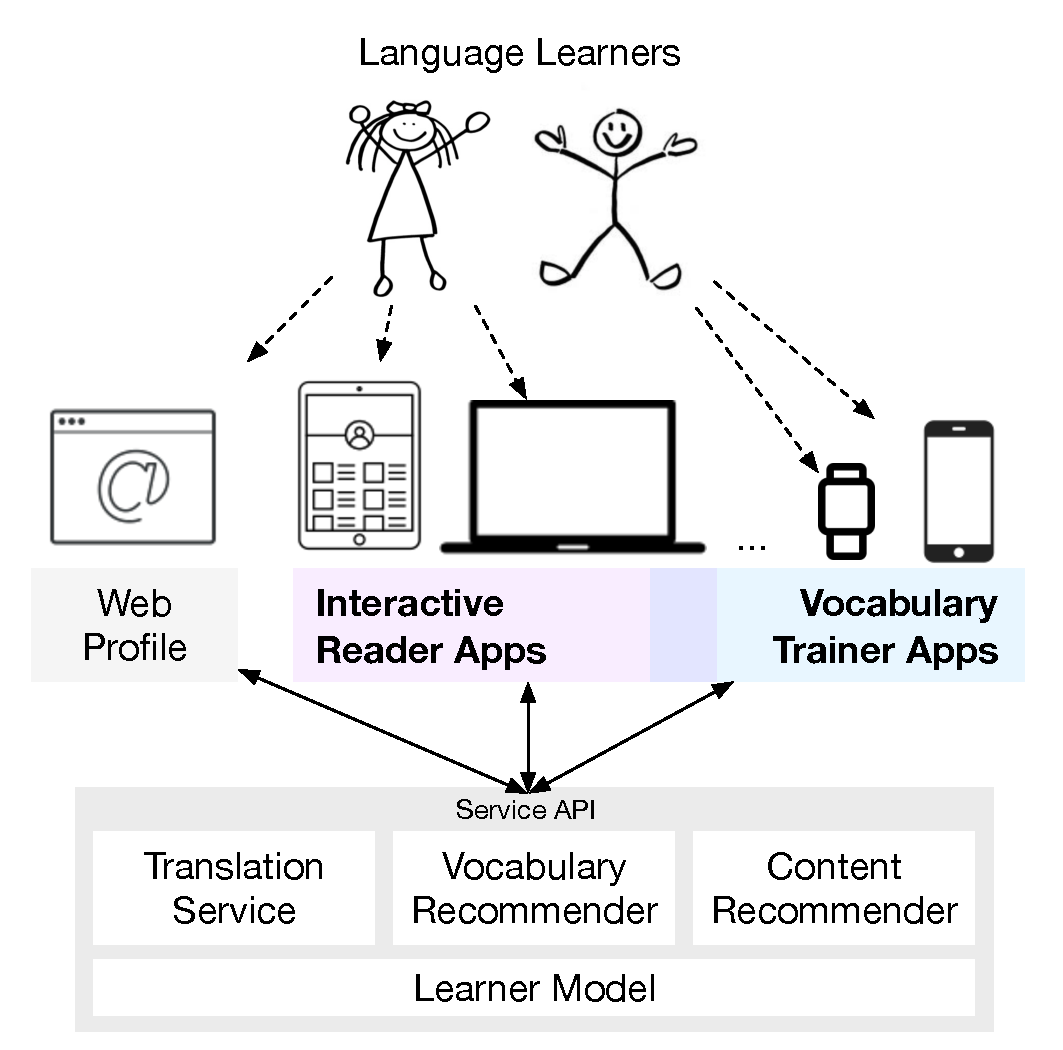
\includegraphics[width=0.75\columnwidth,trim={0 10 0 10},clip]{figures/zeeguu-architecture.pdf}
  \caption{The architecture of the envisioned software ecosystem}~\label{fig:architecture}
\end{figure}

\subsection{Learner Model}

At the core of the ecosystem a {\em learner model} tracks the evolving knowledge. 
Based on this model, algorithms can make recommendations for the individual applications regarding interesting content to read and appropriate vocabulary to study. The individual applications, in turn, report back to the learner model events from which the learner progress can be infered. 

Currently, the model tracks the probabilities of a user knowing words based on interaction events in the apps: asking for a translation, repeatedly encountering a given word without asking for a translation, or answering an vocabulary exercise.


\subsection{The Translation Service}

The Translation Service is a subsystem implemented using Python which provides translations to all the applications in the ecosystem. Instead of implementing our own contextual translation engine, we rely on existing industrial grade translation APIs. To avoid depending on a single service and to also increase the likelihood that at least one of the alternative translations is the correct one, the translation service collects in parallel results from three third party translation APIs: Google Translate, Microsoft Translate, and Glosbe\footnote{Google and Microsoft provide context-aware translations and multi-word translations. Glosbe is a simple dictionary}. \cite{Jager17-mux} In the next section we explain how the best guess is inserted in the text while the alternatives are available for the readers to consult.

The dependency of the translation service on multiple third party APIs allows for a higher reliability and a chance to guarantee a low response time: when a service is down or too slow to respond, the results from it are ignored. We detail elsewhere the strategies we use to keep response times low\cite{Jager17-mux}.

It is critical that the translation service be used by all the applications in the ecosystem since this allows the server to track the words and the context in which they are being looked up. This information is then used for estimating learner knowledge, for generating personalized recommendations, but also for allowing a teacher to gain insight into student activity.


% by interacting with a core API that provides the basic contextual translations, user knowledge estimation, and recommendations for words to be studied and texts to be read \cite{Lungu16}. 

\subsection{Vocabulary Recommender}

The goal of the vocabulary recommender is to program optimally-timed words to practice. 
% 
To schedule the words to practice the system uses an adaptive, response-time-based scheduling algorithm aimed introduced by Mettler et al. \cite{Mettler14-ARTS}. 

% After evaluating several alternative scheduling strategies we settled on the Mettler one since it has been proven to have gains with both familiar, seen items as well as with new, unseen instances and the benefits of adaptive scheduling were present at an immediate test as well as at a delay \cite{Mettler14-ARTS}. 

The words scheduled for practice come from those that are translated by the readers. However, only a subset of words are actually scheduled for practice: those that are deemed {\em fit for study}. Not fit for study are words that can not be found in frequency lists of the language, expressions which are longer than three words, words whose translation is the same as the origin (e.g. digital(en) = digital(de)), and words whose context is too long. 
% A user can force a word to be considered fit for study by {\em starring} it in the user interface.


\subsection{Content Recommender}

The content recommender aims to present the reader with texts that are both interesting and accessible at the same time. The current implementation requires the reader to select online sources (e.g. news, blogs) to be followed. The sources are constantly scanned for the latest articles and cached by using a custom-made library\footnote{Open sourced at: https://github.com/zeeguu-ecosystem/watchmen}. To add a new source, the teacher of the class (or the admin of the system) only has to add the url of the source.
% The user interface for the article selection is presented in the next section. 

The difficulty of a text is computed by aggregating the individual difficulty of its words. Individual word difficulty can vary from 0 to 10 and is computed in the following way: 
% taking into account the ranking of words in the target language based on frequency combined with the past history of a given user's activity: 

\begin{itemize}
	\item When the word is estimated to be known, its difficulty is considered to be zero. A word can be estimated to be known either based on past readings (i.e. encountered multiple times, but never looked up) or based on past vocabulary exercises (i.e. correctly identified in the most recent exercises) 
	\item When the word is in the top 50K most frequent words in the target language, its difficulty is considered to increase with 0.1 for every 500 words; if the word is not in top 50K, its difficulty is ten.
\end{itemize}

With these strategies for computing word difficulty, the text difficulty is computed as the median of the words in the text. One limitation of this measure of difficulty is that it does not take into account the phrase length, as other measures do. \cite{Kincaid75-Readability}


\newpage
\section{A Web-Based Reader and Trainer Platform}
% as we is composed of instantiations of the components. We present them in turn in this section, focusing the discussion on three key activities that a user of such an interactive textbook is interested in: 

% \begin{enumerate}
	% \item finding texts to read
	% \item reading the found texts
	% \item practicing vocabulary in context
% \end{enumerate}

 % interacts with: the reader and the trainer applications. 
% \begin{added}
	
	In this section we present the user interface of the prototype {\em personalized language textbook} that we have built. It combines in a single responsive web application a reader applications and a vocabulary trainer with multiple exercise types, and thus, can be used from a variety of devices. In the user evaluation reported in this paper, it was used from Windows, Android, and iOS devices. Although not presented here, since it was not used in the user evaluation, a smartwatch application also exists as another vocabulary trainer \cite{Nien16-time}.

% \end{added}




%!TEX root=paper.tex

% \newpage
% \subsection{Web Article Reader}


    % A basic text reader should allow the learners to find interesting texts (e.g. news, blogs) and should provide a facile interaction for reading and translating unknown words. 
  
% The Web Article Reader allows the learners to subscribe to various sources of articles (e.g. news, blogs) and provides a facile interaction for reading and translating unknown words. 
% It consists of several components:

\subsection{Finding Personally Interesting and Accessible Texts}
% personally relevant vs. interesting... relevant can mean both interesting and not too difficult. 
% \ml{make sure that we use source consistently in the text; not feed for example.}
% From the user's point of view, the Reader is organized around {\em sources\xspace} of articles. The system categorizes sources by their language. 
The current system allows the learners to subscribe to various online sources (i.e. news, blogs) and then monitors those sources for new texts. Figure \ref{fig:system_subscriptions} presents the source subscription dialog listing multiple text sources for French.
% multiple sources for every language are pre-loaded in the system and if a reader wants to add a new source they have to send an email to the maintainers of the system. 



    \begin{figure}[h!]
    \centering
      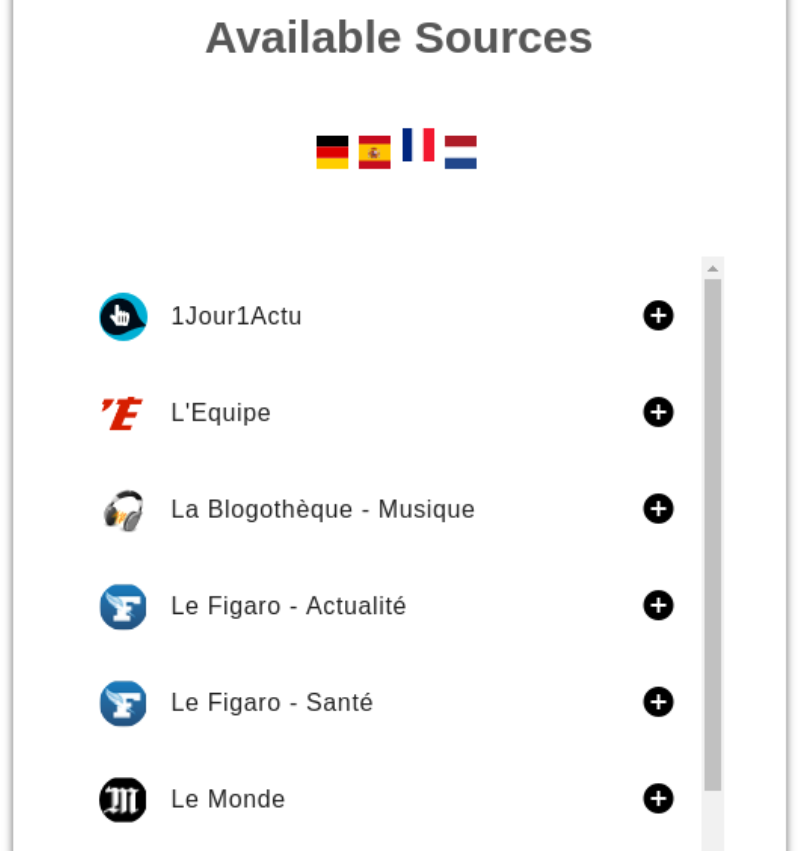
\includegraphics[width=0.40\columnwidth]{figures/available_sources_short}
      \caption{Different users subscribe to different sources}~\label{fig:system_subscriptions}
    \end{figure}

% A multi-lingual learner can subscribe to multiple sources in different languages. 
% \begin{added}

  Once a reader is subscribed to a source, that source is constantly monitored for new articles, which are recommended to the learner in an article browser like the one in Figure \ref{fig:article_listing}. The browser displays for each article an icon representing its source, a title, a summary, and an estimated difficulty level.
  To visualize the reading difficulty of an article, there are three levels of information displayed: 1) a flag representing the language of the article since a learner could be actually registered to feeds in multiple languages; 2) a color coded difficulty from green to yellow to red, to  allow the user to rapidly judge difficulty on an intuitive level; 3) a numerical difficulty score  to allow a more quantitative judgment of the estimated difficulty.
    
% \end{added}

    \begin{figure}[h!]
    \centering
      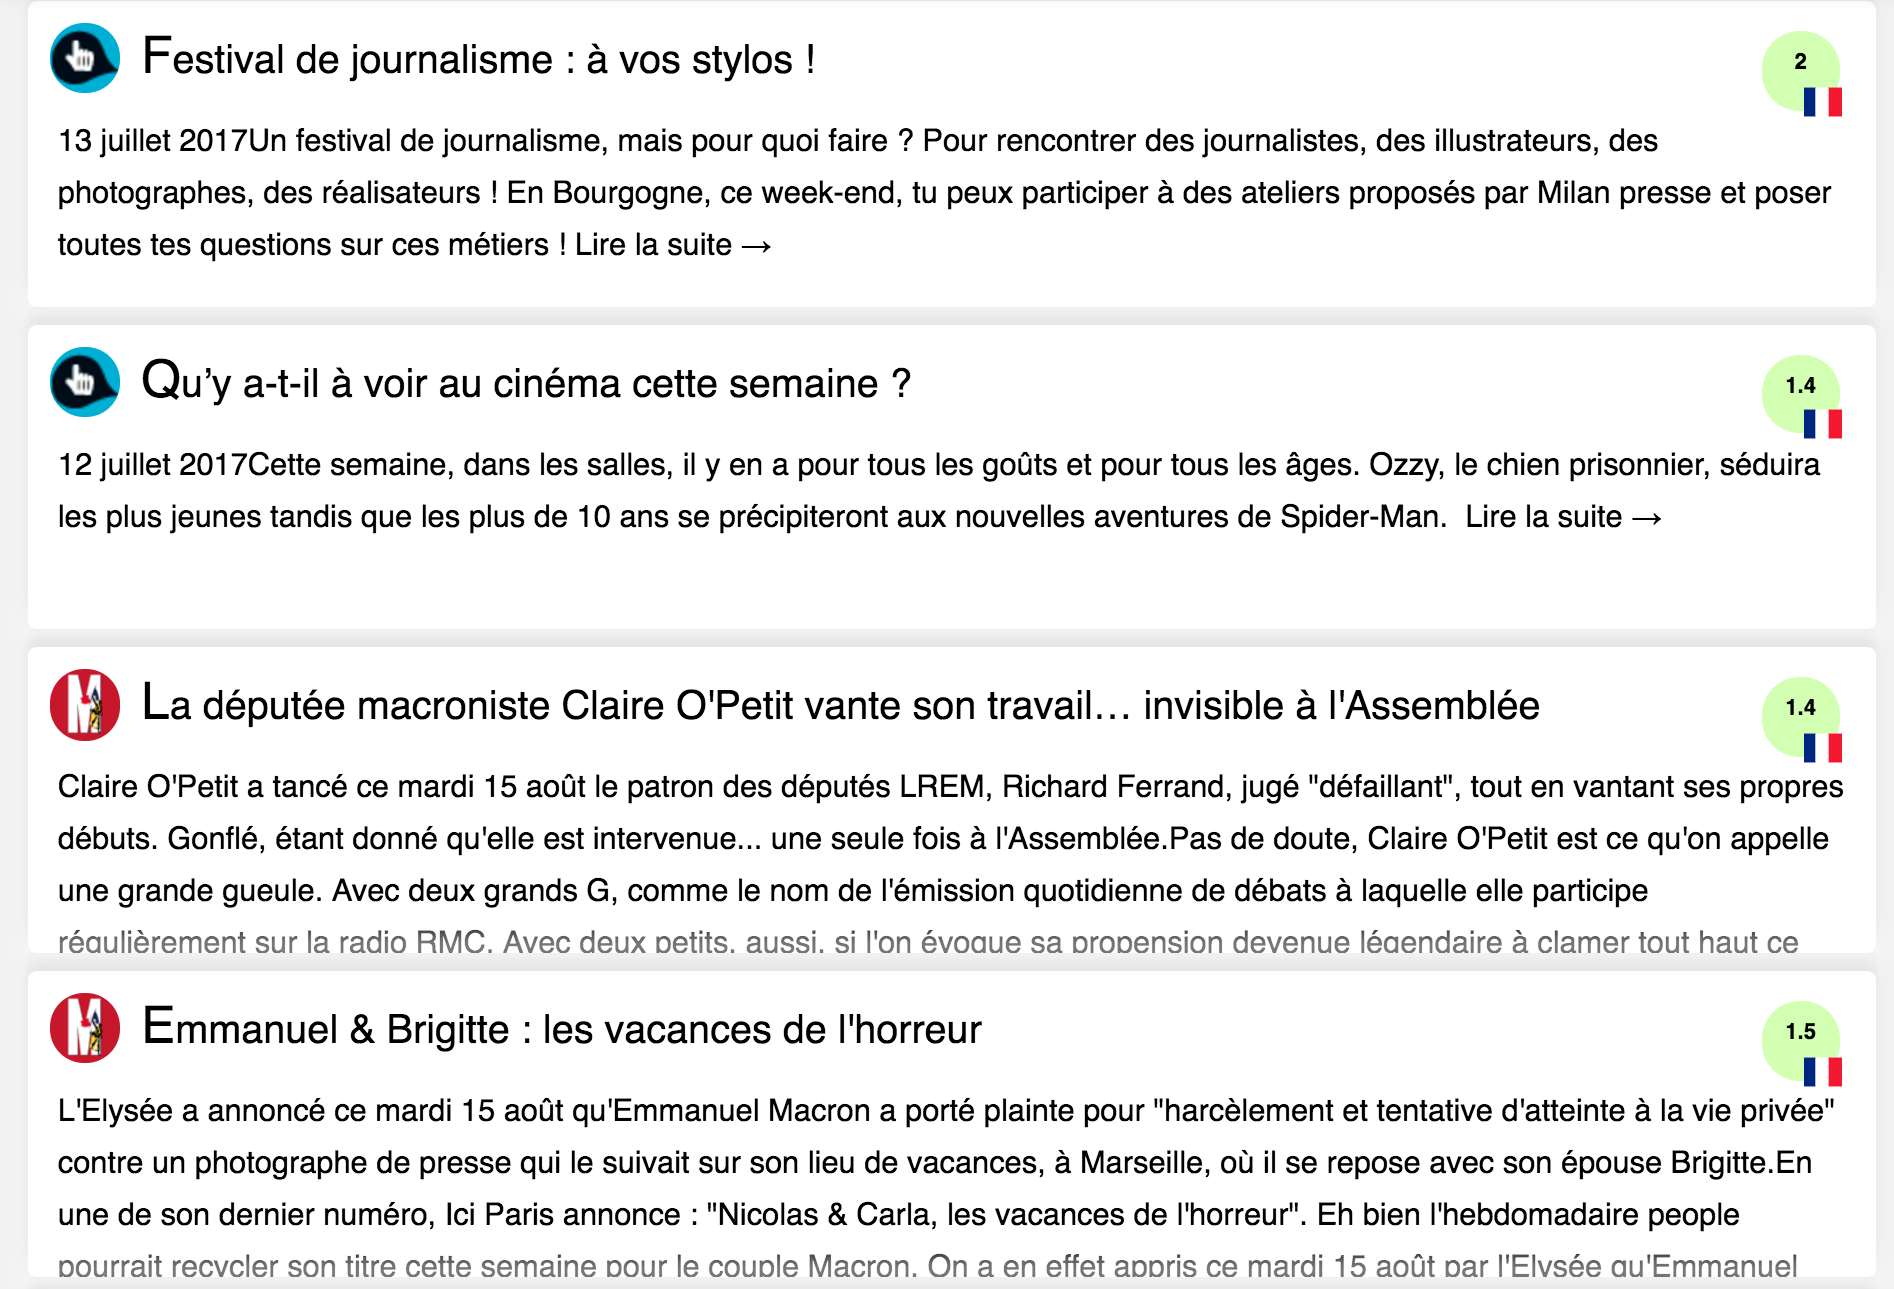
\includegraphics[width=0.95\columnwidth]{figures/article_listing_short}
      \caption{Article browser presents estimated difficulty levels }~
      \label{fig:article_listing}
    \end{figure}



% Difficulty estimation takes into account the frequency of the vocabulary items in the text. The system filters out articles that are too difficult given that it was deployed with non-advanced learners.\footnote{This is one of the limitations of the system that we discuss later.}

\subsection{Interacting With Unknown Words While Reading}
% Reading Texts to Understand

To make reading as facile as possible, the reader is optimized for the most frequent action that a reader is likely to want to perform: translating a word. Thus, when a user clicks on a word, a translation is inserted right after the word, as Figure \ref{fig:translated_word} illustrates\footnote{A screencast is at \url{https://vimeo.com/250152073}}: 

\begin{figure}[h!]
\centering
  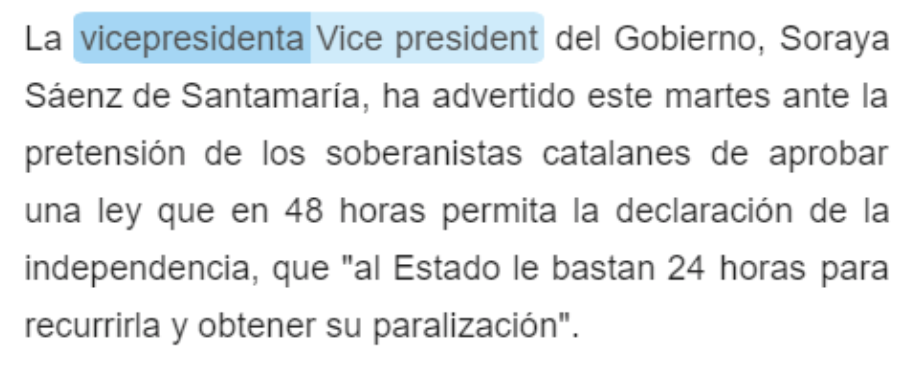
\includegraphics[width=0.75\columnwidth]{figures/translated_word}
  \caption{A translated word is inserted after the tapped word.}~\label{fig:translated_word}
\end{figure}

Two other alternatives that we explored and eventually dropped (for each had disadvantages) were: 

\begin{enumerate}

  \item Temporarily showing a popup of the translation and then hiding it again. This had a disadvantage for difficult sentences, where multiple words must be translated. The reader can forget translated words by the time they arrive at the end of an article, requiring them to re-translate.
  \item Using the native selection mechanism to select text as opposed to click / touch. 
  % We experimented with allowing the learner to select a word in the same way this is normally done on the corresponding platform. 
  This had the disadvantage that native selection is not designed as a priority action and thus is slow to respond (e.g. on Android a user must hold their fingertip down for almost a second before the contextual menu is displayed). 
\end{enumerate}


\subsubsection{Translating Multi-Word Expressions}

The user can chain a few consecutive words into a single translation by simply tapping adjacent words which are then automatically merged in a translation bubble (Figure \ref{fig:translation_extension}). This is useful for collocations and in cases where by expanding the translated set of words the precision of the translation increases. 

    \begin{figure}[h!]
    \centering
      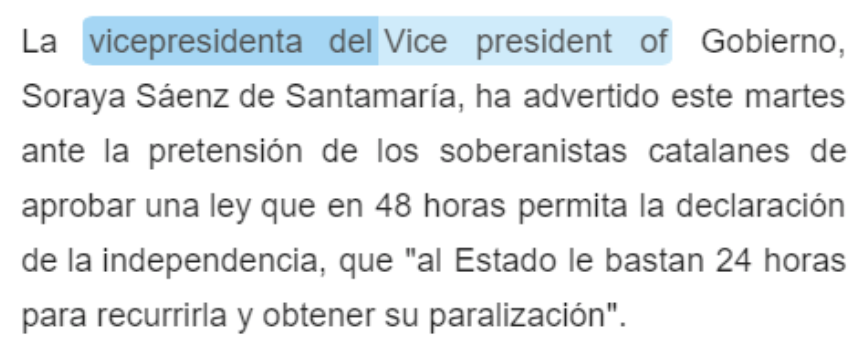
\includegraphics[width=0.75\columnwidth]{figures/translated_words1}
      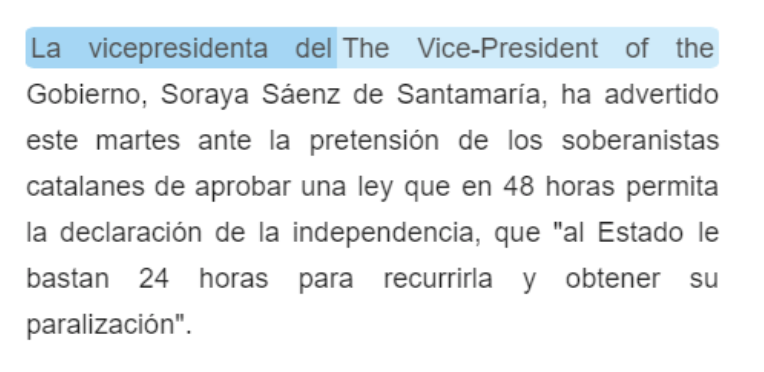
\includegraphics[width=0.75\columnwidth]{figures/translated_words2}
      \caption{When adjacent words are tapped the translation bubble is extended accordingly}~\label{fig:translation_extension}
    \end{figure}

This minimalistic interaction model serves a double purpose - it enables and eases the translation of several chained words but it discourages users from translating entire sentences or phrases. This is in line with the recommendations of the literature (e.g. Renandya argues that extensive reading should discourage intensive use of translations\cite{renadya07-power}) but also because it reduces the amount of characters which are being translated by the learner (and thus the costs of the system, since some of the translation services have a per-character fee). 

One of the limitations of this interaction is that it is not clear (at least at the moment) how to expand it for the situations in which expressions are present that are composed of words which are not adjacent (e.g. particle verbs in German).


\subsubsection{Compensating for the Limits of Machine Translation}
Due to the limitations of machine translation multiple translations might be possible in a given context. In such a case the system will insert the most likely alternative as described earlier right after the selected text, but it will allow the reader to discover alternatives. With a click on the translation, a drop-down menu appears in which alternatives are presented. Figure \ref{fig:registrations} shows that besides the predefined alternatives the learner can provide their own translation via an input box (the third line, ``took place'' is typed in by the learner in the figure). 


\begin{figure}[h!]
\centering
  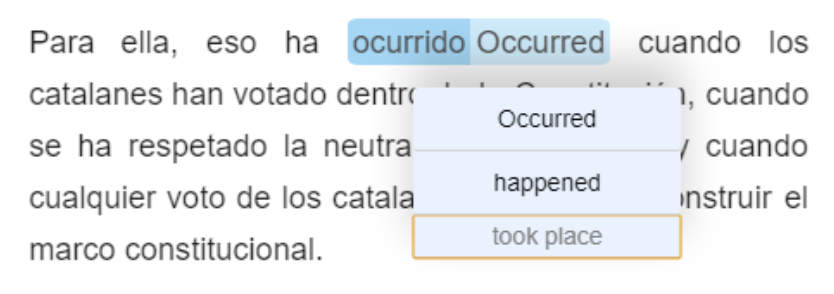
\includegraphics[width=0.75\columnwidth]{figures/translation_alter_menu}
  \caption{A translated word is inserted after the tapped word.}~\label{fig:registrations}
\end{figure}

\subsubsection{Discovering the Pronounciation of a Word}

The process we followed while developing the reader was an iterative process, with short release cycles (one or two weeks), and frequent testing with members of the research team, and the occasional external user. 

One of the features that we added following a suggestion of an early beta-tester -- a teacher of Dutch as a foreign language -- was the pronounciation of a translated word. After exploring several trade-offs between flexibility, ease of use, and a clean user interface, we settled on triggering the pronounciation of a word (or group of words) with a tap. 

% The pronounciation is generated by using the HTML5 Speech API which is supported by most modern browsers both on the mobile and on the desktop. 

% \ml{could ask the users if they are happy with it.}
% Although no user has yet complained about it, this means that a user can not pronounce a word without it being translated first. It might also be that for some languages this is more important than for others, and we just did not have users learning those languages (e.g. Danish is notoriously hard to pronounce). In the future we plan to expand the interaction modes to allow pronounciation to exist seperately from translation.
%!TEX root=paper.tex

% \newpage
\subsection{Practicing Personalized Vocabulary in Context}

% Given the list of words that a user looked up -- and are thus likely to be unknown -- we can generate exercises for them. 
Given that the translation API captures the context together with every translation, exercises can be personalized for every user based on their past reading by using the original context in which the words have been encountered.

Figure \ref{fig:exercise_translate} shows such a generated exercise which asks the reader to translate a given word in the context in which it was encountered in a past reading. The main interactive elements (IEs) that are specific to this exercise are an input box that allows the user to enter a solution (IE5); a button for checking the correctness of the input answer (IE2); a hint button which presents the correct answer (IE1). Two types of control that span exercise types are: a word pronunciation option (IE3) and a feedback option (IE4) which allows the user to provide feedback about the exercise.

\begin{figure}[h!]
\centering
  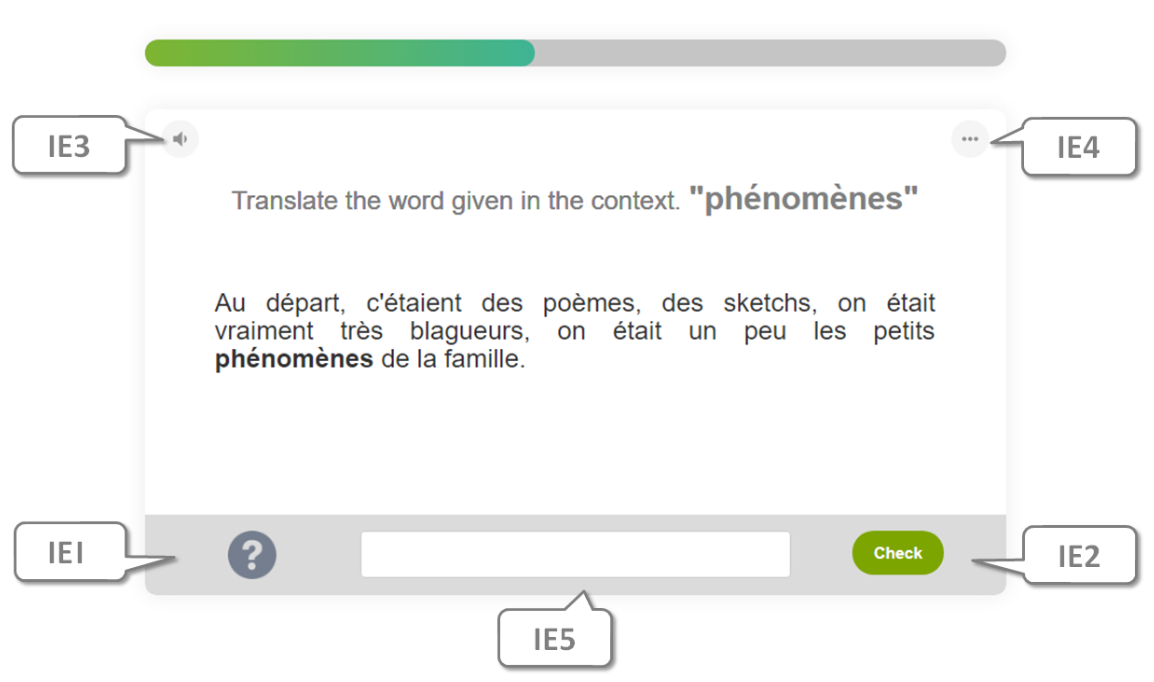
\includegraphics[width=0.9\columnwidth]{figures/exercise_translate}
  \caption{Translate exercises ask the user to translate a word in a given context (retrieved from the user's past readings)}
  \label{fig:exercise_translate}
\end{figure}

	The system currently implements three other types of vocabulary practice exercises\footnote{Detailed description of the exercise types are elsewhere\cite{Avagyan17a-blocks}}, which can be split into two categories: 
\begin{enumerate}
	
	\item Free text input -- where the text must be typed in the learned language (exercise type: Find)

	\item Multiple choice -- where the user is presented with a set of alternatives (exercise types: Choose, and Match). 

\end{enumerate}

% \subsubsection{Selecting Words to Study}

Since a learner might encounter many words that are not understood, we need to prioritize those that are to be studied in exercises. We use two aspects to prioritize words: 

% The words good for study are the ones that are either starred by the user, or are important and of quality based on a set of heuristics. 

\begin{enumerate}

  \item Word Importance. The system prioritizes words based on the frequency with which they appear in the language.\footnote{For word frequencies we use frequencies computed based on movie subtitles which have been shown to be highly representative to frequencies in human interacitons \cite{New07-subtitles}}. 
  
  \item Context Quality. The system favors words that come with a context which is not too short but not too long. 

\end{enumerate}




% \subsection{Translator Service}

% The core API of the ecosystem provides translations. The main advantage of this indirection is that this allows the server to track the words that are looked up and the context (sentence) in which they are being looked up. This information is then used for estimating learner knowledge and for generating personalized exercises. 

% The Translation Service is an API implemented using Python. Instead of implementing our own contextual translation engine, we decided to rely on existing industrial grade translation APIs. To avoid depending on a single service and to also increase the likelihood that at least one of the alternative translations is the correct one, the translation service dispatches in parallel requests to at least three third party translation APIs: Google Translate, Microsoft Translate, and Glosbe. \cite{Jager17-mux} The first two provide contextual translations and multi-word translations, while the third is a simple dictionary. 

% The dependency of the translation service on multiple third party APIs allows for a higher reliability and a chance to guarantee a low response time: when a service is down or too slow to respond, the results from it are ignored. We detail elsewhere the strategies we use to keep response times low\cite{Jager17-mux}.


% \begin{figure}[h!]
% \centering
%   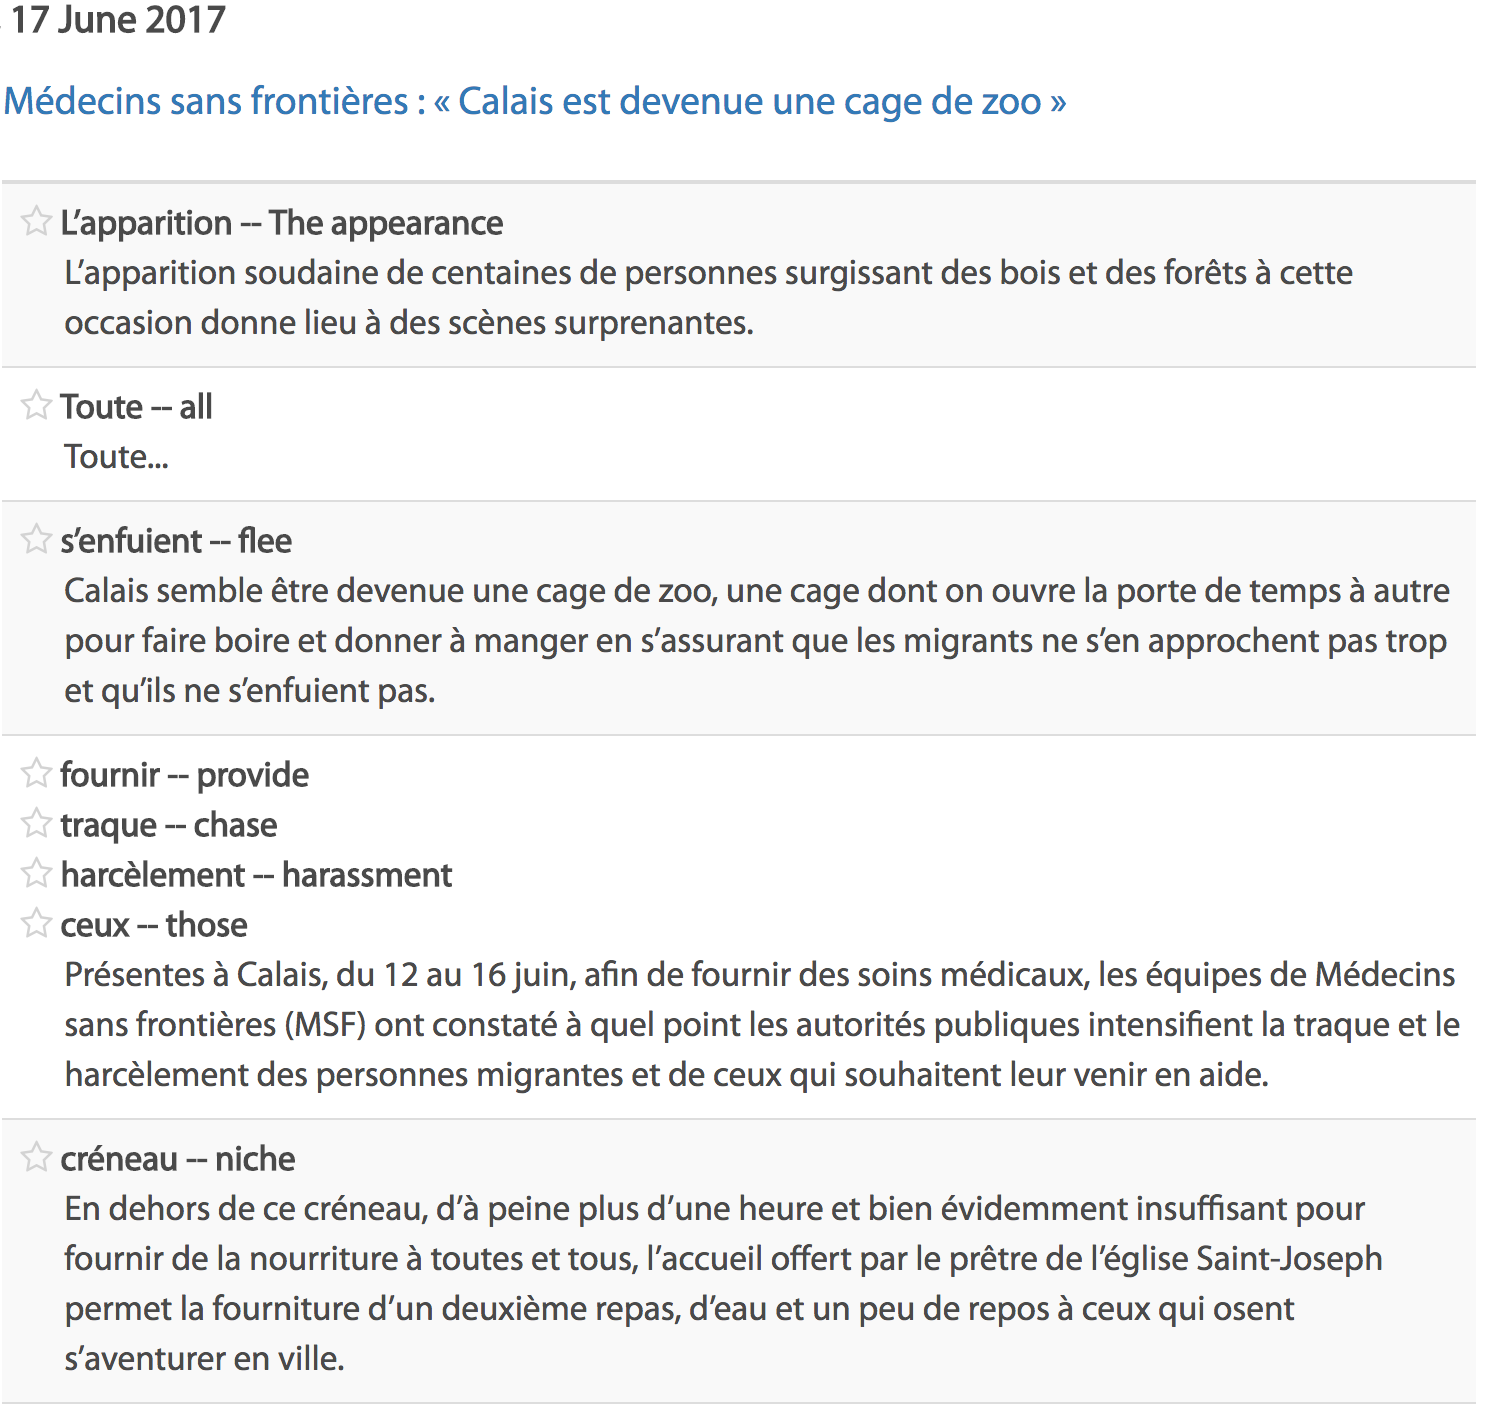
\includegraphics[width=\columnwidth]{figures/teacher_dashboard.png}
%   \caption{A teacher can see the log of the words that a student looked up, their chosen translations, and the corresponding contexts}{
%   \label{fig:teacher}
%   }
% \end{figure}





%!TEX root=paper.tex

% \newpage
\section{Testing The System With High School Students}
\label{sec:demographics}

We tested our system with \stcnt students from a public highschool in Netherlands, representing three classes that have the same French teacher and are bilingual in Dutch and English. All the students are below eighteen.

% \begin{added}
{\bf Usage Scenario. }
	The teacher asked the students to use the system for {\bf supplementary reading}. 
	% , aside from the other activities that were done in the class. 
	He encouraged them to read texts they found interesting and to build up their own {\em personalized portfolio of words}, complementary to the list of mandatory words that were common in every class.
	
	For every half an hour of usage, the students had to write a brief report on how they spent their time and submit it to the teacher. The teacher could then decide to selectively test them on the basis of their reports. 
	% This was a requirement from the teacher and based on a strategy 
	The teacher had used this strategy in the past with other software that he used in class. 
	% This might have affected negatively the willingness of the students to spend time on the platform.
% \end{added}


{\bf Deployment.} At the beginning of June 2017 we introduced the system and its usage to each of three classes. With few exceptions the students created an account and started using the system the latest on June 9th and until the end of the month, which coincided with the end of the study year. 
% \begin{added}
Students used personal computers and Android/iOS devices.
% \end{added}

Before creating accounts on our platform, we asked the participants to answer a survey about their current level of knowledge, learning strategies, and reading interests. A handful of the participants, who were not in class when we presented the system, did not fill in the survey.

When asked whether they have favorite topics they would like to read about, half of the students mentioned various topics while the other half did not answer the question. From the topics that they mentioned as possible interests some of the more popular were: sports, music, travel, lifestyle, fashion, movies, and somebody mentioned as interest {\em ``no politics''}.


In collaboration with the teacher we seeded the system with a variety of French news and blogs that cover the aforementioned aspects: 1Jour1Actu, L'Equipe, La Blogoteque, Le Figaro, Le Monde. 
% 
% \begin{added}
	% 
	Even if the source of readings was not actually the entire web, practically, having many dozens of news articles daily (only Le Figaro has usually more than forty in a day) offers sufficient opportunity for the free choice of individually interesting articles. 
	% {\em reading personalization} 
	% We could have added even 
	
% \end{added}



We deployed the system with the translations to English since, based on our experience translation APIs are of higher quality when one of the languages is English and because the students and their teacher were comfortable with the idea.\footnote{We told the students to ask if they want their account switched to Dutch. None of the students requested this.}

We also invited the students to send us feedback at any time if they encounter problems or if they have ideas for improvement. Several of them did email. Towards the end of the month, we deployed several in-app focused pop-up questions using a customer opinion elicitation service called HotJar. After the month was over we sent out a follow-up questionnaire.


% \subsection{The Teacher Dashboard}

We also provided the teacher with a dashboard to see the activity of the students: the texts that were read and translations they requested. This chronological activity view is available also for the student who can solely see their own history.


% \begin{figure}[h!]
% \centering
%   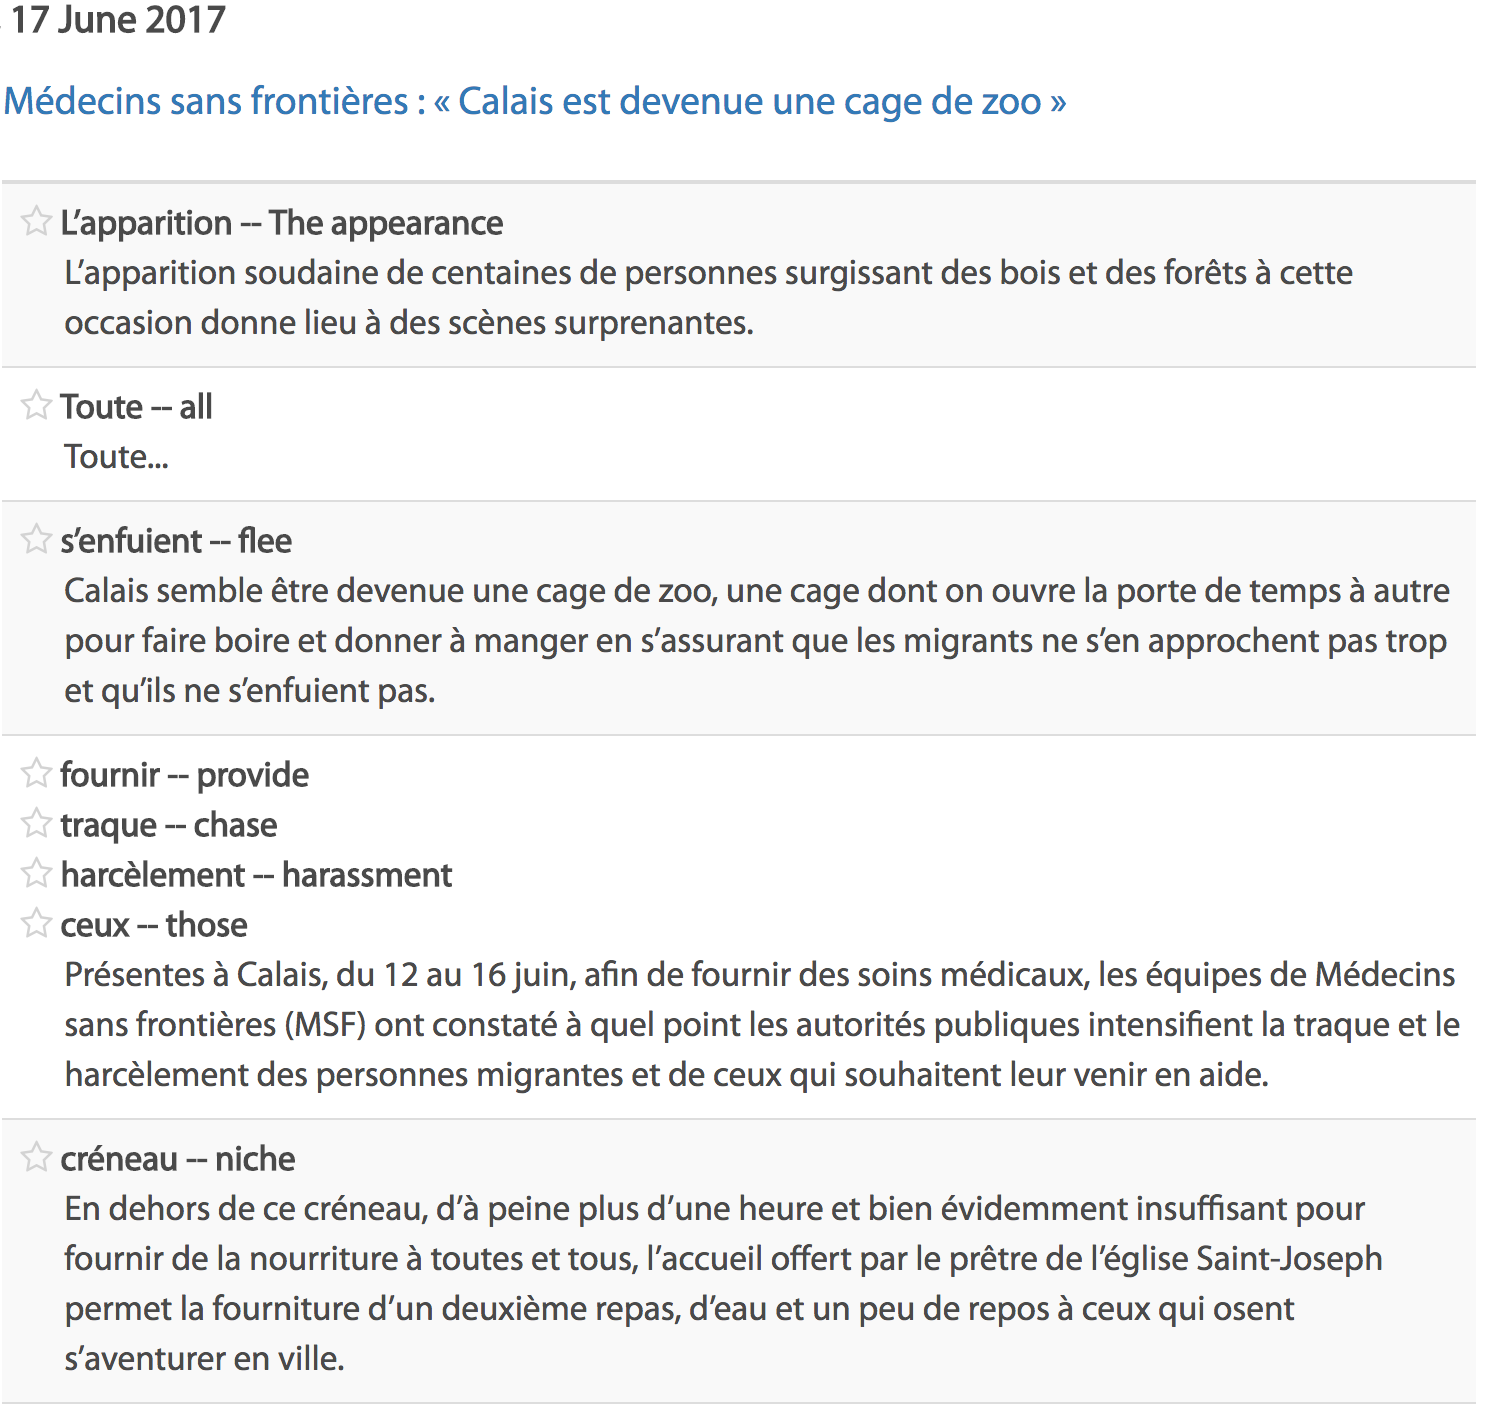
\includegraphics[width=0.8\columnwidth]{figures/teacher_dashboard.png}
%   \caption{A teacher can see the log of the words that a student looked up, their chosen translations, and the corresponding contexts}{
%   \label{fig:teacher}
%   }
% \end{figure}





{\bf Demographics.} 
The participants that filled the survey were 54 female and 15 male with ages below 18. Based on their self characterization, 53 students are level B1 (i.e. can understand the main points of clear standard speech, can narrate an event or experience) and 16 are level A2 (i.e. can describe their surroundings and communicate immediate needs). 

{\bf Usage.}
% There were a total of 221 distinct login-days to the system\footnote{We do not have the actual logins, so if a user logs in multiple times in a day, we count that only once.}. 
In average a student logged in on 2.83 different days\footnote{We can not tally the actual logins, so if a user logs in multiple times in a day, we count that only once.}(median 2.5). The most active student used the system in 8 different days while 19 students used it in a single day. The students interacted with 279 articles in total for an average of 5 and median of 3 articles each. The average number of words translated by the students is 71 and median 70. In total, during the entire duration of the study students solved 14,609 vocabulary exercises with a median of 85 exercises and a maximum of 2,865.













% To talk to Nienke about the other types of analysis we can do on this data
%!TEX root=paper.tex


%!TEX root=paper.tex

\newpage
% \section{How Is Reader Personalization Being Used?}
\section{How Is Reading Personalization Being Used?}
% \section{How Do Learners Use Reader Personalization?}
% \section{How Do Students Use the Possibility of Reading Personally Interesting Articles?}
\label{sec:results}


% \subsection {Feed Subscriptions}
Figure \ref{fig:subscriptions} represents an incidence matrix in which the columns represent students and the rows represent article sources. If a student is registered to a given source, the intersection of the respective row and column is a $\Diamond$. 
% 
We would expect to see full horizontal rows of data-points if every user subscribed to a given feed, and full vertical rows if every user subscribed to all of the feeds available. The absence of such patterns proves that different individuals prefer to subscribe to different sources.

% The figure illustrates that giving the students the freedom to choose the sources they wanted, allowed each one of them to express their interest. 

\begin{figure}[h!]

\centering
  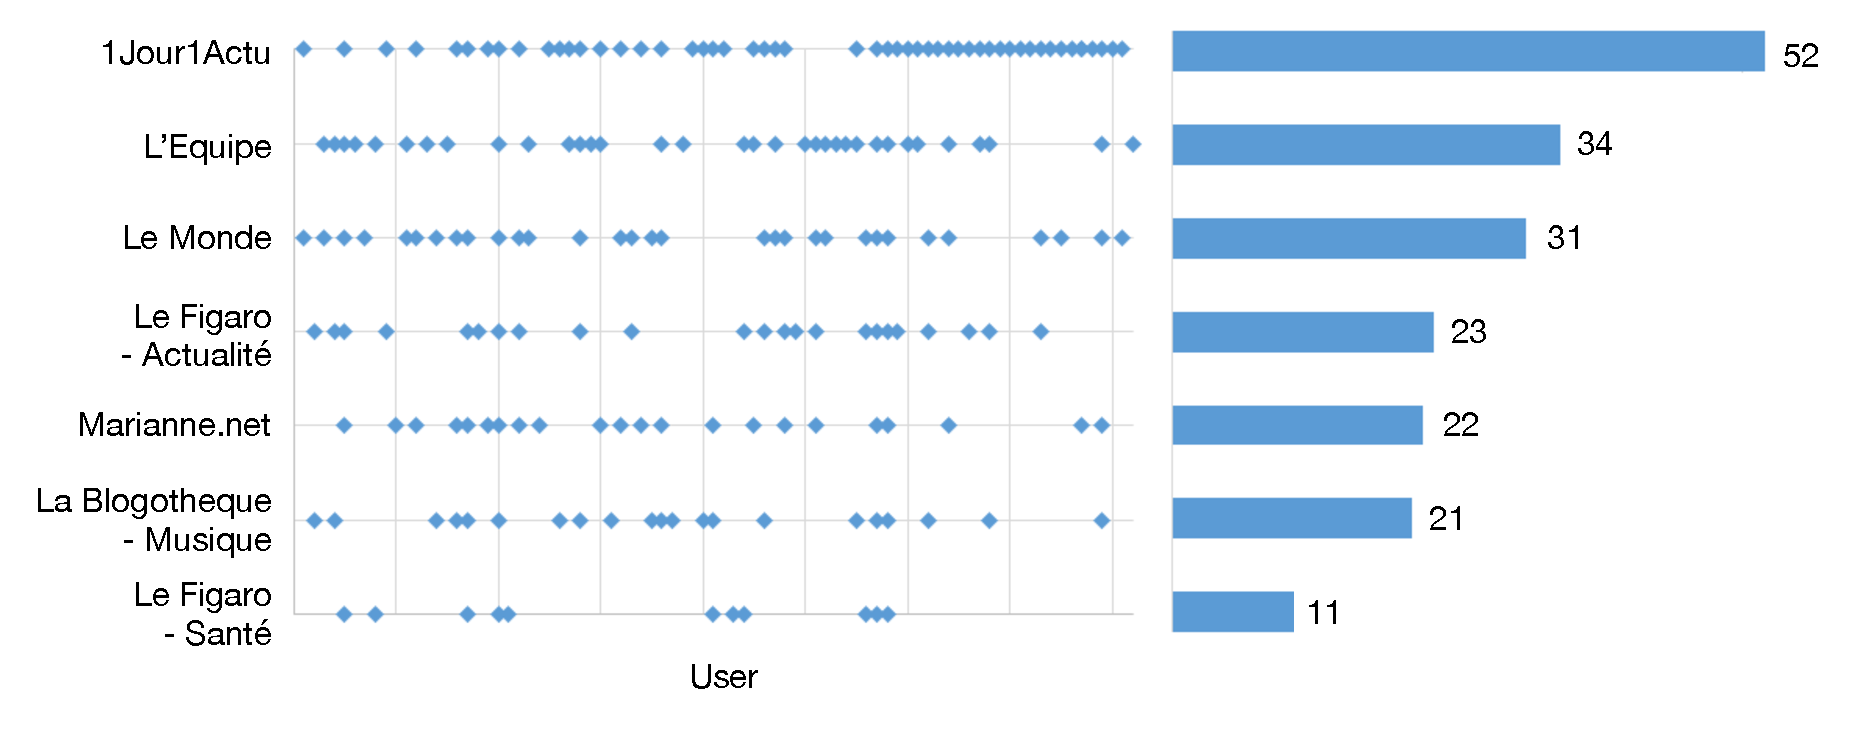
\includegraphics[width=\columnwidth]{figures/subscriptions}
  \caption{Different students subscribe to different sources}
  \label{fig:subscriptions}  
\end{figure}

Projecting the data points onto the horizontal axis results in the histogram to the right of Figure \ref{fig:subscriptions} which shows that source popularity varies. 
% Projecting the data- points onto the horizontal axis and sorting the results results in the histogram in Figure \ref{fig:feedpopularity}.
% 
% \begin{figure}[h!]
% \centering
%   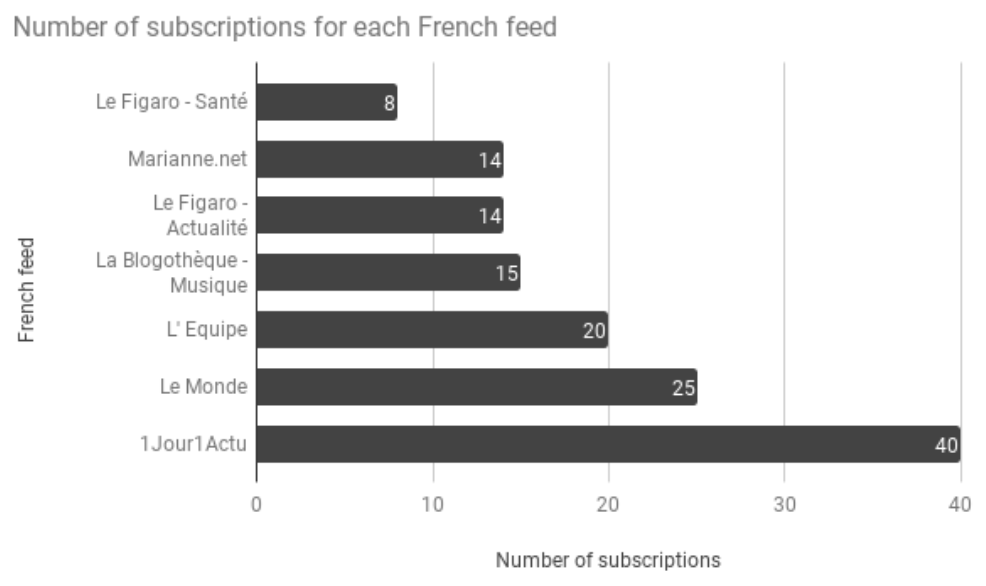
\includegraphics[width=0.85\columnwidth]{figures/feed_popularity}
%   \caption{Some feeds are more popular than others}
%   \label{fig:feedpopularity}
% \end{figure}
% {\em 1Jour1Actu} is the most popular article source and Le Figaro - Sant\'e is the least. 
To show that popularity is not related to the order in which they are presented in the subscription dialog, Figure \ref{fig:popularityvsranking} compares the popularity order with display  order. 
% One can see how the second-to-last presented feed, Le Monde, is the second most popular feed by measure of subscriptions. Conversely, the feed listed above Le Monde is actually the least subscribed-to feed in our listing.


\begin{figure}[h!]
\centering
  %!TEX root=paper.tex
\newcommand{\picscale}{0.45}
\newcommand{\yunit}{0.5}
\begin{tikzpicture}[scale=\picscale, every node/.style={scale=\picscale},font=\sffamily]
    % Columns.
    \node at (0  , 0) {\bf Presented};
    \node at (2.5, 0) {\bf VS};
    \node at (5  , 0) {\bf Popularity};
    
    % As presented.
    \node at (0,-1*\yunit) {1Jour1Actu};
    \node at (0,-2*\yunit) {L'Equipe};
    \node at (0,-3*\yunit) {La Blogoth\`{e}que};
    \node at (0,-4*\yunit) {Le Figaro - Actualit\'{e}};
    \node at (0,-5*\yunit) {Le Figaro - Sant\'{e}};
    \node at (0,-6*\yunit) {Le Monde};
    \node at (0,-7*\yunit) {Marianne.net};
    
    % As popular.
    \node at (5,-1*\yunit) {1Jour1Actu};
    \node at (5,-2*\yunit) {L'Equipe};
    \node at (5,-3*\yunit) {Le Monde};
    \node at (5,-4*\yunit) {Le Figaro - Actualit\'{e}};
    \node at (5,-5*\yunit) {Marianne.net};
    \node at (5,-6*\yunit) {La Blogoth\`{e}que};
    \node at (5,-7*\yunit) {Le Figaro - Sant\'{e}};
    
    % Arrows between presented and popular.
    \draw [->] (1,-1*\yunit)   --   (4,-1*\yunit);
    \draw [->] (1,-2*\yunit)   --   (4,-2*\yunit);
    \draw [->] (1.2,-3*\yunit) --   (3.7,-6*\yunit);
    \draw [->] (1.6,-4*\yunit) --   (3.4,-4*\yunit);
    \draw [->] (1.4,-5*\yunit) --   (3.7,-6.9*\yunit);
    \draw [->] (1,-6*\yunit)   --   (4,-3.1*\yunit);
    \draw [->] (1.2,-7*\yunit) --   (3.9,-5*\yunit);
    
\end{tikzpicture} 
  \caption{The popularity of the feeds vs. their ranking in the UI}
  \label{fig:popularityvsranking}
\end{figure}



% \subsection{Article Interactions}
Figure \ref{fig:articles_read} shows an incidence matrix of users (columns) and articles that they interact with (rows). 
The distinct column patterns hint at the fact that each user explores their own interest:
  a few students read exclusively articles about sports (e.g. one student read twelve articles only about sports), 
  one student reads exclusively articles about health;
  nobody reads on all the topics but the majority read on multiple ones.

% , and there is no one article that is interesting for all. 
% The vertical ``line'' in the figure's left half represents an over-active reader.
% \begin{added}
  % Interacting with means that the user translated at least one word in that article. to check with Dan that this is the definition! we currently do not have information about whether a user read the article to the end. 
% \end{added}
% 
% \begin{added}
% 
  % After investigating the reading patterns of students we observed that there are those who enjoy reading a variety of topics, but also those who like to read a single topic. 
  % From the latter category we mention:
 % \cite{renadya07-power}.
  % \begin{itemize}
  %   \item one student who has read twelve articles exclusively on topics about sports in five different days
  %   \item one student who has read six articles exclusively about health topics over two distinct days
  %   \item TODO: Add discussion about some students who have a more omnivorous taste, and thus, also read much more.
  % \end{itemize} 


    % The student \#657 in the published dataset has read 10 articles exclusively about sport in three different days between June 7 and July 4th. 
  
% \end{added}

\begin{figure}[h!]
\centering
  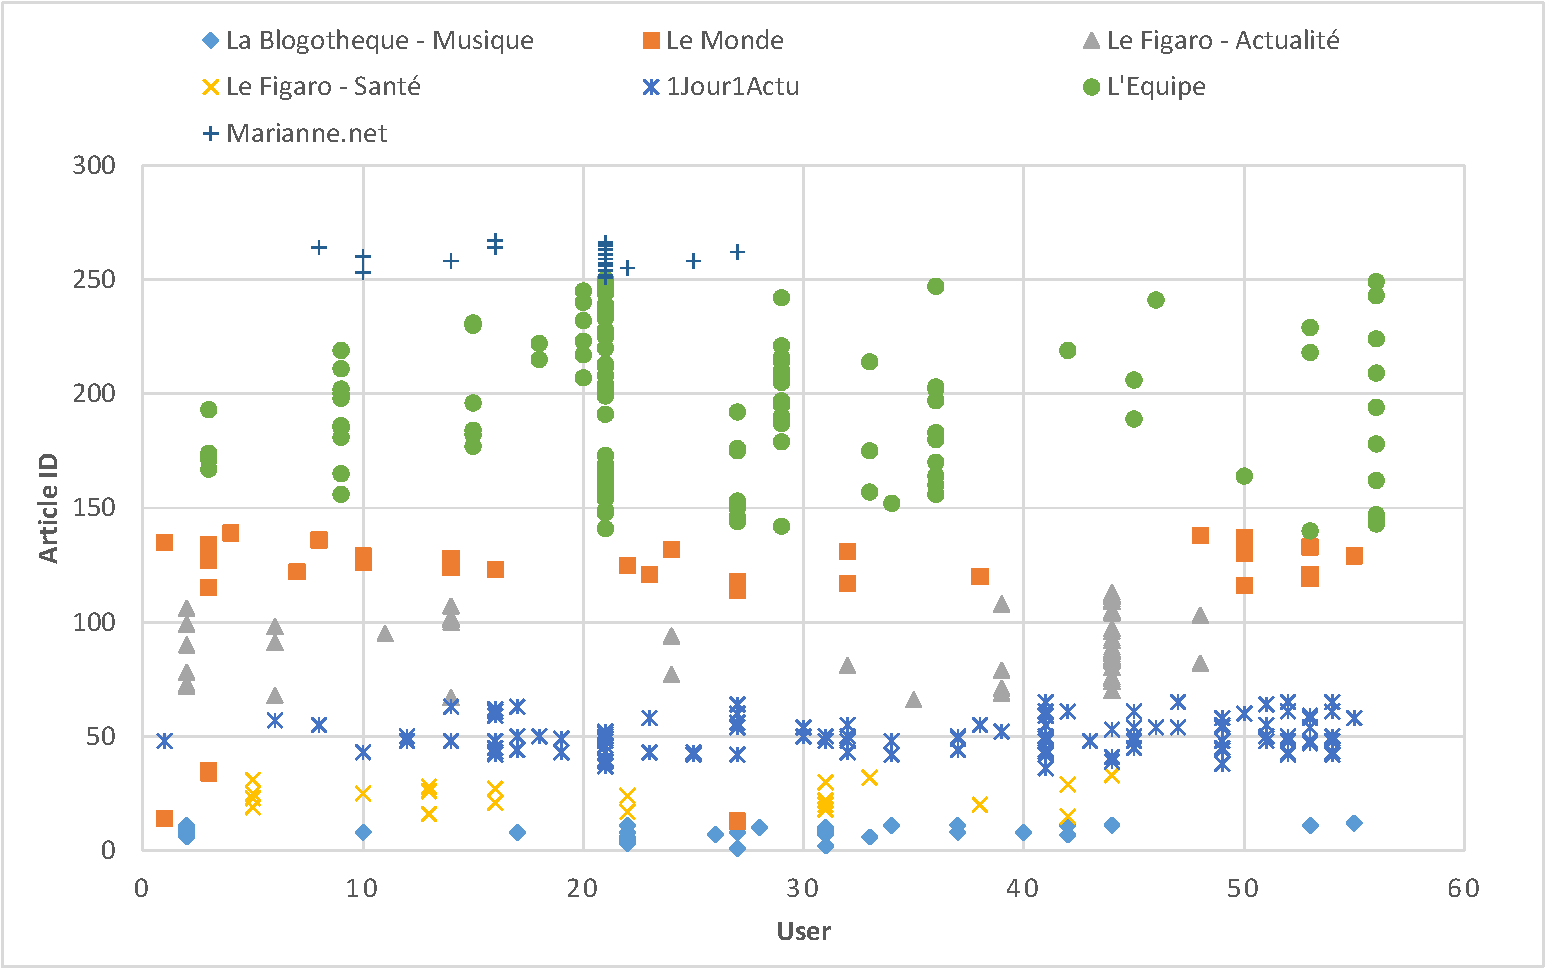
\includegraphics[width=\columnwidth,trim={24 20 40 20},clip]{figures/users_articles_color}
  \caption{Each student (column) reads a different article mix}~\label{fig:articles_read}
\end{figure}


%!TEX root=paper.tex

\newpage
% \section{How Do Students Improve Their Vocabulary?}
% \section{How Does The System Help Students Improve Their Vocabulary?}
% \section{What Is The Impact of the System on the Learner Vocabulary?}
% \section{Does The Vocabulary of the Learners Improve?}
% \section{Do Students Improve Their Vocabulary?}
\section{Is There an Impact on Student Vocabulary?}

  The value of extensive reading can be found, besides the new words that are learned, in the strengthening of the knowledge of the existing words, increased fluency, and increased grammar knowledge. Some of these benefits can be reliably measured only after a time longer than our deployment \cite{renadya07-power}. 

  However, since our system combines free reading with vocabulary exercises and tracks all word interactions, by analyzing the learner interaction with the reader and the exercises\footnote{A more detailed analysis can be found elsewhere \cite{Avagyan17a-blocks}}, we can provide a glimpse into two measures of progress visible after one month of usage: increasing confidence about words and learning new words. 

   \begin{figure}[h!]
  \centering
    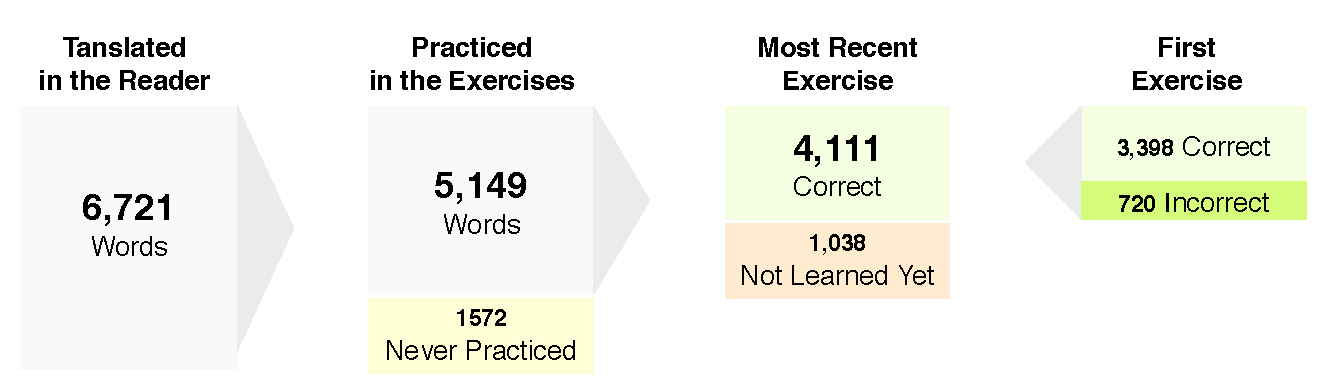
\includegraphics[width=0.9\columnwidth,trim={0 10 0 15},clip]{figures/word-learning-flow.pdf}
    \caption{Word encounters in the Reader and Exercises}
    \label{fig:word_learning_flow}
  \end{figure}

  Figure \ref{fig:word_learning_flow} summarizes the interactions of the students with words in the reader and the exercises. The figure is based on the analysis of the user interaction database and shows that: 

  \begin{itemize}
    \item From the 6,721 words that were looked up in the reader, 4,759 were used in the exercises platform. Since the learners requested a translation, they were either not sure about these words or did not know their meaning.

    \item More than 1,900 words were not practiced in the exercises. 
    Some did not get their turn to be scheduled by the algorithm and others were not presented because the system deemed them not fit for study (cf. Vocabulary Recommender, p.3). 
    % Given that not all the words can be practiced, this is an argument for prioritizing the words that the students are presented with in the exercises.

    \item For 3,626 words 
    % (76\% of all the words present in exercises) 
    the learners were able to correctly identify them the latest in the last associated exercise. Out of these: 

    \begin{itemize}
      \item 3,261 words 
      % (68\% of all the words in exercises) 
      were recognized already for the first time in the exercises. These are {\bf words likely to be strengthened by translating while reading}: the students were unsure when encountering them initially in the reader but eventually recognized their meaning when encountering them later in the exercises\footnote{It could also be that the students learned them after the first encounter in the text, but we keep the more conservative hypothesis}.  They represent 48\% of all the words that the students translated in the reader.

      \item 365 words 
      were wrong during their first exercise interaction but were correct in the final one. These {\bf words are likely to be learned via the exercises} by the students. \footnote{This number is conservative. We consider an answer to be correct only if it was right from the first attempt, without the use of a hint, and without typos.}

    \end{itemize}

  \item For 1,133 words 
  % (24\% of all the words present in exercises) 
  the outcome of the final exercise that involved was not a correct answer. Thus we assume that they were {\bf still not learned at the end of the experimental period}. Some of them might have been learned after the last exposure via the testing effect \cite{Roediger11-TestingEffect}, but we can not be sure.

  \end{itemize}

% \end{added}


% \newpage
% \section{How Are The Reader Features Used?}
\section{How Do Learners Interact With the Reader?}
% \section{What Is The Relative Importance of the Various Interaction Modes?}
\newcommand{\feature}[1]{{\em #1}}
The reader interaction is more innovative and complex than the exercises.
This is why we use telemetry to investigate how do learners use the features of the reader. 

Telemetry has been successfully used for understanding user behavior in games \cite{Gagne11-telemetry} but also more generic contexts, such as automatically detecting personas from large scale interaction data \cite{Zhang16-telemetry}. In our study, we used telemetry to track the usage of various relevant features in the reader of the personalized textbook in order to better understand the usage of our system.

Based on logging every interaction of every user, Figure \ref{fig:feature_usage} (left) shows the six most used features of the system.\footnote{An extended analysis that includes more features is elsewhere. \cite{Chirtoaca17-apollo}} Figure \ref{fig:feature_usage} (right) shows the number of distinct users for each category of events. A larger number of distinct users indicates a feature that is more important to the students. 

  \begin{figure}[h!]
  \centering
    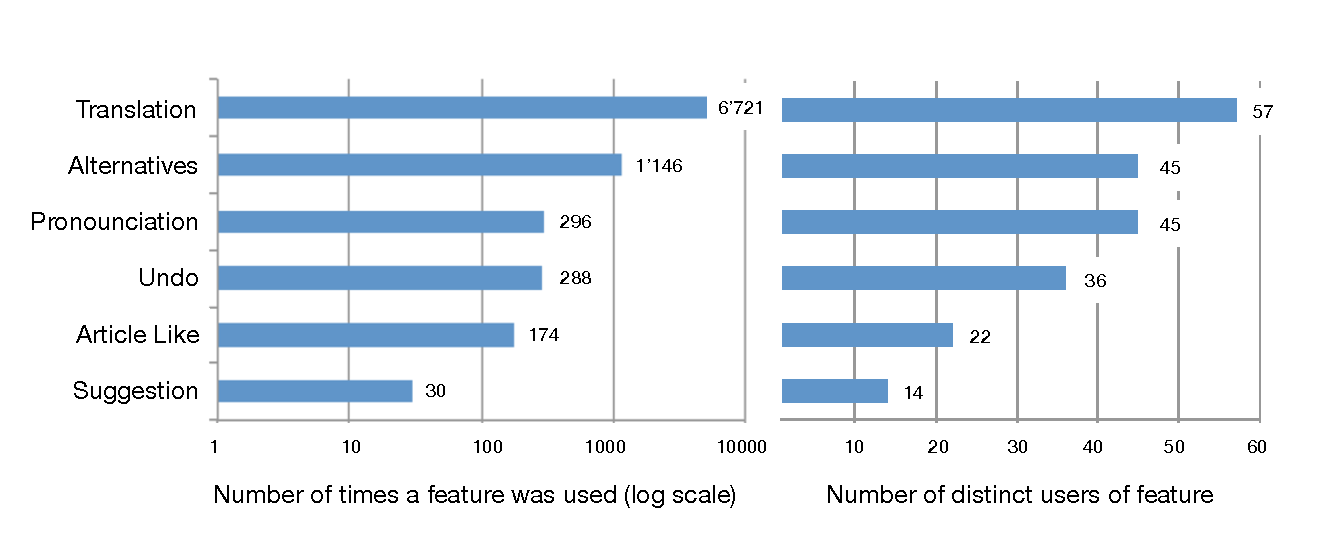
\includegraphics[width=1.0\columnwidth]{figures/feature-usage}
    \caption{Popularity of features by their recorded usage-events (left) and number of users that use them at least once (right)}
    \label{fig:feature_usage}
  \end{figure}

% With 6.700 occurrences, 
\feature{Requesting a translation} is the most used interaction of the system and \feature{showing translation alternatives} is the second most used one. The six-to-one ratio between the two features (6,721 to 1,146 as in Figure \ref{fig:feature_usage}) is an indicator of the limitations of the automatic translation. The fact that they are both achievable with one click or touch proves to have been a good decision. 
 % -- these are probably the situations when learners ask for 

\feature{Pronuncing a word} is he third most used interaction. On average, there are about 1.66 pronunciations for a given translation, suggesting that users are often asking for a second pronunciation after hearing it the first time. 

% \ml{@dan, do you agree with this conclusion? it's opposite to your thesis, but I think this is the correct interpretation}

% In addition, we looked at the number of times the same word or phrase was pronounced by the same user. This data ranges from one single pronunciation to 14 pronunciations for the same word (phrase). The size of this interval is mostly due to the users' different proficiency in a certain language and the difficulty in pronunciation of the word (phrase) itself. Nevertheless, on average, the number approaches 1.66 pronunciation requests for the same piece of text, suggesting that users are generally sufficiently content with a pronunciation after hearing it the first time.


\feature{Undo-ing a translation} is used when the user wants to remove the last translation that was inserted in the text. For the proposed interaction mechanism this feature seems useful. 

\feature{Liking} an article that was just read by clicking the corresponding button at the bottom of an article happened 174 times. This information can be used in the future to improve article recommendations.
 % and maybe to add a social dimension to the system by providing information about how other people react to a given article.

\feature{Suggestion of an alternative} allows users to contribute their own translations when they are not satisfied with the one automatically provided by the system. This interaction is used seldom and by only a minority of users. It still is to be determined whether this is due to readers being satisfied with the automatic translations and their alternatives, or due to a low involvement. It might also be that more advanced readers would benefit more from this feature.
% \ml{which brings me to: @Dan, what do you mean by alternatives here? :) Is it the number of times somebody selected an alternative, or the number of times they opened the menu. In any case, can we get the other number?}

  % \begin{figure}[h!]
  % \centering
  %   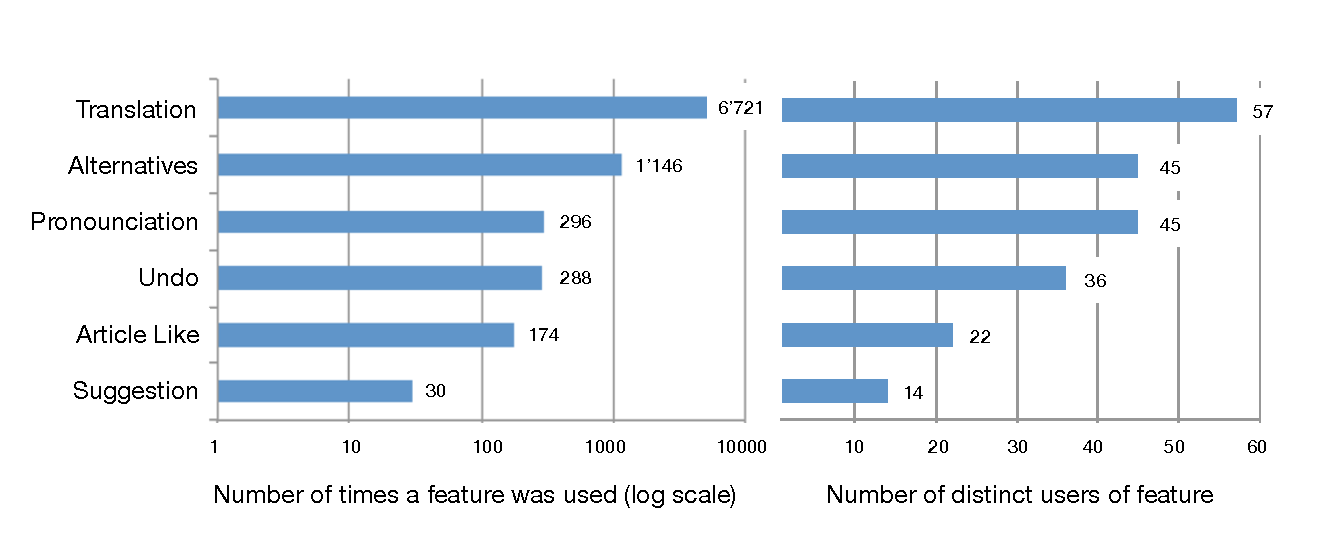
\includegraphics[width=0.6\columnwidth]{figures/feature-usage}
  %   \caption{The usage of the various reader features by the various users }
  %   \label{fig:usage_per_user}
  % \end{figure}


%  We see that: 
% \begin{itemize}
%   % \item Not all the users of the system use translations
%   % \item \feature{Translation suggestion} is used by very few users. It still is to be determined whether this is due to readers overwhelmingly being satisfied with the automatic translations and their alternatives, or due to a low involvement. 
% \end{itemize}




\newpage
\section{How Do Students Interact With Exercises?}

The system presented four types of vocabulary practice exercises to the students. In total, during the entire duration of the study we observed 18,082 attempts being submitted by the students in 14,609 exercises\footnote{Attempts include wrong submissions, and requests for hints}. Figure \ref{fig:ex_interactions} presents the number of answers which had a ``correct'' outcome (red) vs. exercises which had a ``wrong'' outcome (blue). The figure shows one student who submitted 2,865 answers during one month, and about six eager students who submitted about  700 answers each. 

  \begin{figure}[h!]
  \centering
    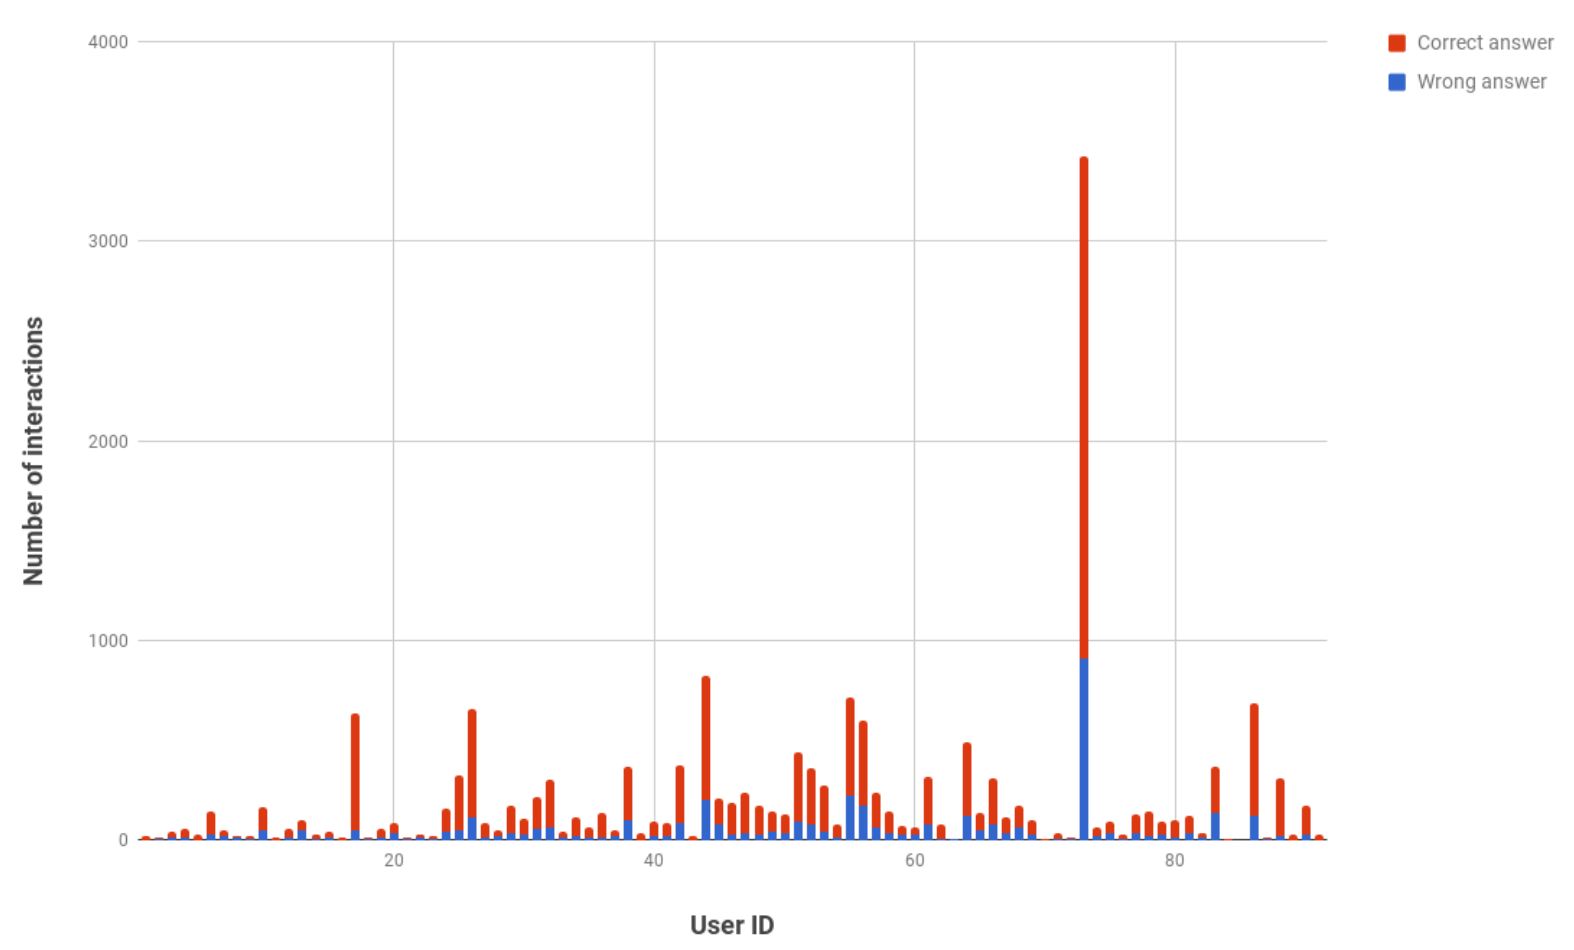
\includegraphics[width=0.9\columnwidth]{figures/exercise_interactions_count.png}
    \caption{Correct (red) and wrong (blue) exercise outcomes per student}
    \label{fig:ex_interactions}
  \end{figure}

The figure does not include one other type of outcome, {\em requesting a hint}, which is presented in the table below grouped per exercise type. The corresponding number of hints suggests that the multiple-choice exercises (i.e. Match, Choose) are simpler than free text entry exercises (i.e. Find, Translate).

\begin{tabular}{lrrrr}
  % source id: 
  % choose -- 5
  % find -- 4
  % translate -- 7
  % match -- 6
                      & Choose  & Find & Translate & Match \\ \hline
  Total attempts  & 7,180    & 6,249 & 2,643      & 2,010\\
  Hint requests       & 29      & 529  & 847       & 16 \\ \hline
  \label{tab:hints_per_ex_type}
\end{tabular}

Figure \ref{fig:activity_per_day} shows the days when learners practice exercises. The x-axis has the days of June and the y-axis has the different user ids. The figure suggests that the students are doing exercises at their own pace over the observed period. The activity is rather sparse, with a more intensive period towards the end 

  \begin{figure}[h!]
  \centering
    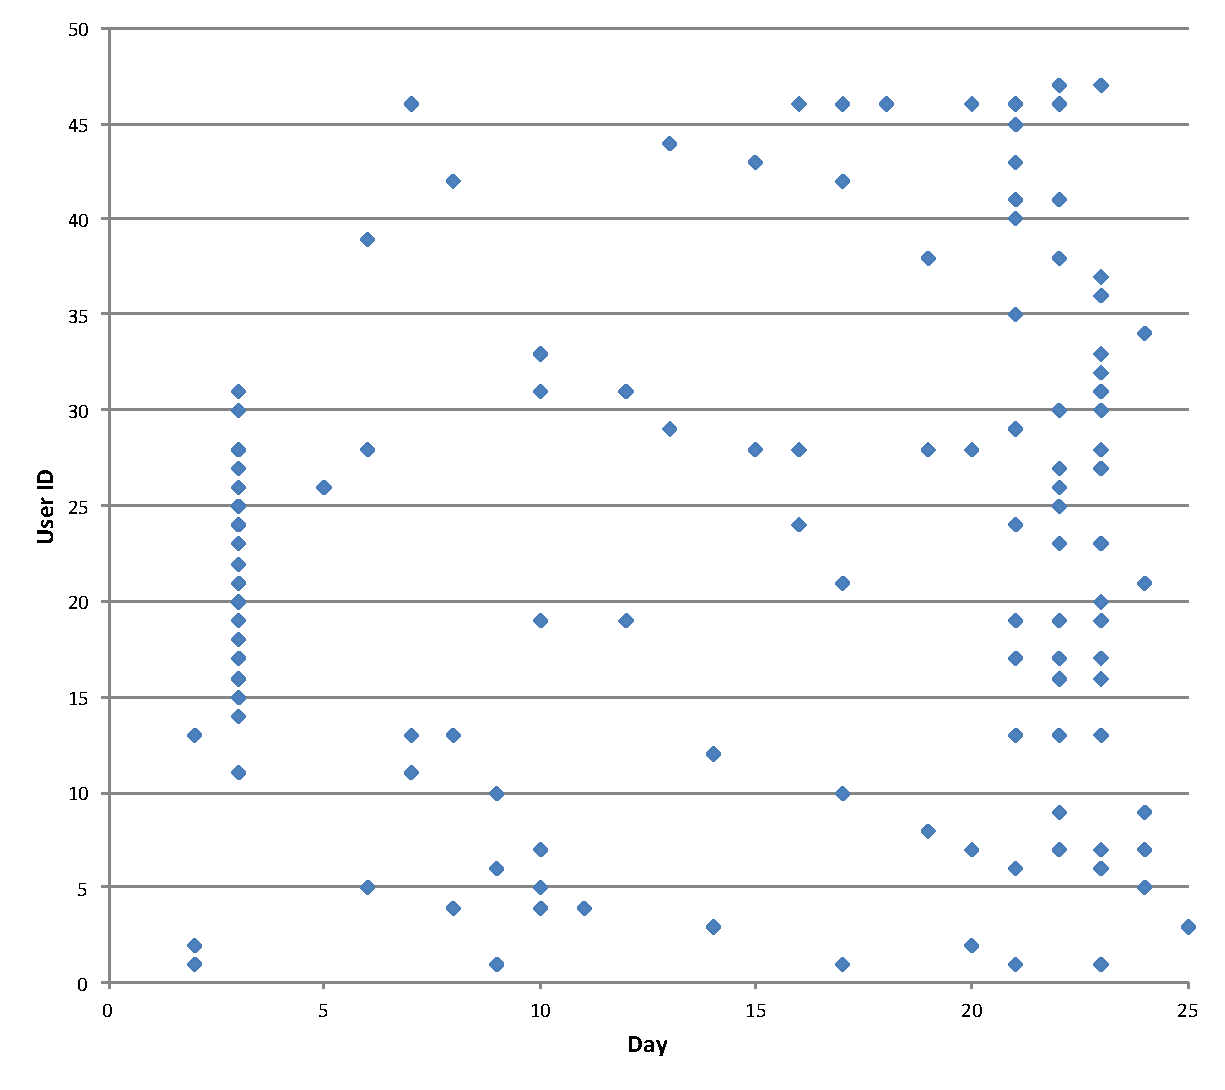
\includegraphics[width=0.7\columnwidth]{figures/user_exercise_activity_vs_day.pdf}
    \caption{The students are doing exercises at their own pace throughout the one month interval }
    \label{fig:activity_per_day}
  \end{figure}


% % \begin{added}




% \newpage
% % \section{How Do Students Improve Their Vocabulary?}
% % \section{How Does The System Help Students Improve Their Vocabulary?}
% \section{What Is The Impact of the System on the Learner Vocabulary?}

%   The value of extensive reading and vocabulary practice can be found, besides the new words that are learned, in the strengthening of the knowledge of the existing words, increased fluency, and increased grammar knowledge. Some of these benefits can only be clearly measured after a longer time \cite{renadya07-power}. 

%   However, since our system combines free reading with vocabulary exercises, by analyzing the learner interaction with the reader and the exercises we can provide a glimpse into two measures of progress visible after one month of usage: {\em increasing confidence about words} and {\em learning new words}. 

%    \begin{figure}[h!]
%   \centering
%     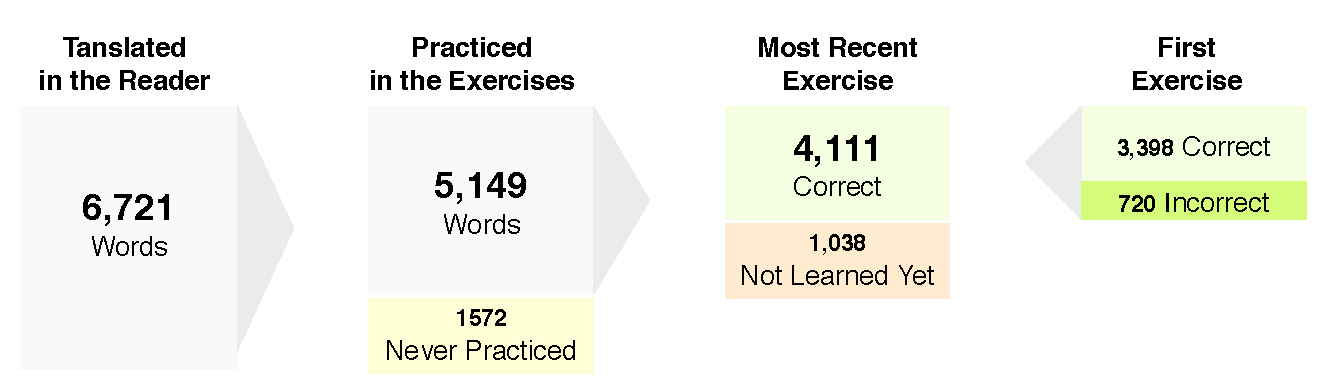
\includegraphics[width=0.9\columnwidth]{figures/word-learning-flow.pdf}
%     \caption{An overview of the words encountered in the Reader and practiced in the Exercises}
%     \label{fig:word_learning_flow}
%   \end{figure}

%   Figure \ref{fig:word_learning_flow} summarizes visually the interactions of the students with words in the reader and the exercises parts of the system. The figure is based on the analysis of the user interaction database and shows that: 

%   \begin{itemize}
%     \item From the 6,721 words that were looked up in the reader, 5,149 were used in the exercises platform during the learning period. Since the learners requested a translation for these words we can assume that they were not known to the readers or at least the readers were unsure about their meaning. 

%     \item More than 1,500 words were not practiced in the exercises. Some of these never got the chance to be scheduled by the algorithm and others were not presented to the students because the system decided they were not interesting enough. 
%     % Given that not all the words can be practiced, this is an argument for prioritizing the words that the students are presented with in the exercises.

%     \item For 4,111 words (80\% of all the words present in exercises) the learners were able to correctly identify the meaning in the last associated exercise. Out of these: 

%     \begin{itemize}
%       \item 720 words (14\% of all the words in exercises) were wrong during their first exercise interaction but were correct in the final one. These {\bf 720 words are likely to be learned via the exercises} by the sixty students in our study. They represent 10.75\% of all the words that the students translated in the reader.

%       \item 3,391 words (66\% of all the words in exercises) were recognized already for the first time in the exercises. These are {\bf likely to be words for which the knowledge was strengthened by using the system}: the students were unsure when encountering them initially in the reader but eventually recognized their meaning when encountering them later in the exercises. 
%     \end{itemize}

%   \item For 1,038 words (20\% of all the words present in exercises) the outcome of the final exercise that involved them showed an incorrect answer. Thus we can assume that they were {\bf not learned at the end of the experimental period}.

%   \end{itemize}

% % \end{added}















%!TEX root=paper.tex

\newpage
\section{What is the Perception of the Learners?}
\label{sec:perception}

\subsection{About The Reader}

After the semester was over, we sent an email asking the students to answer the survey about their experience and received \surveyrespondents answers. Figure \ref{fig:reader_use} summarizes the answers to the first question that asked the respondents to rate the ease of use (top) and usefulness (bottom) of the reader. 

 \begin{figure}[h!]
    \centering
      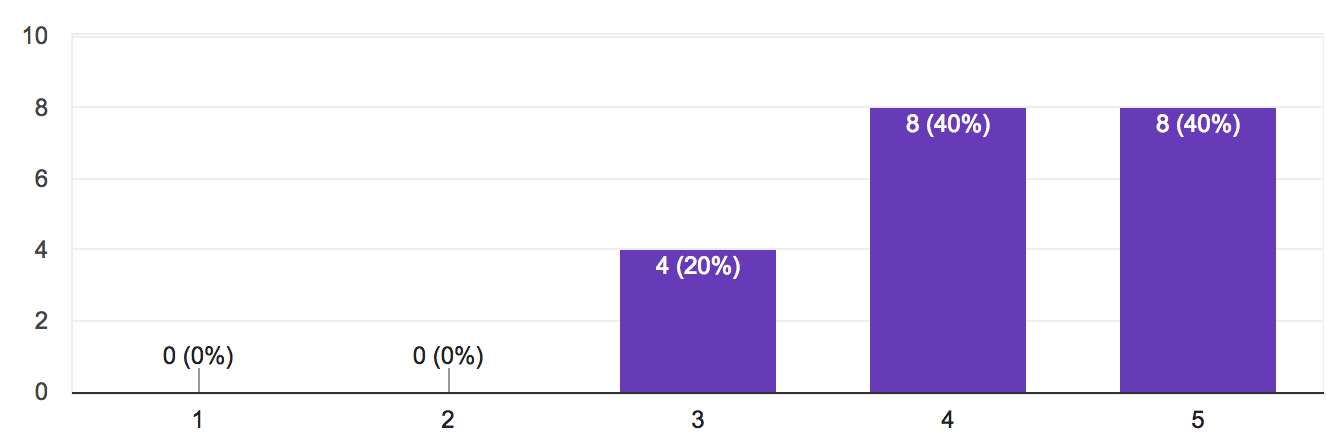
\includegraphics[width=0.8\columnwidth]{figures/opinions/reader_ease_of_use}
      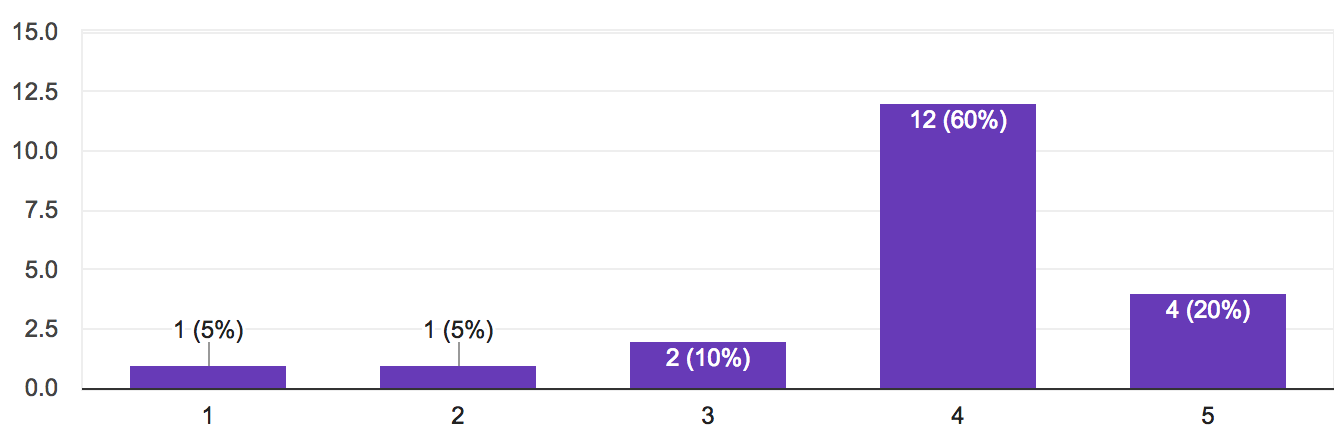
\includegraphics[width=0.8\columnwidth]{figures/opinions/reader_usefulness}
      \caption{Feedback on Reader ease of use (top) and usefulness (bottom)}
      \label{fig:reader_use}
    \end{figure}

When asked what would make their experience with the Reader better many of the students thought that the system was good the way it was and few had some very specific features in mind (e.g. night reading mode\footnote{Complete feedback available in the GitHub repository of the paper.}). There was however, one request which was expressed multiple times, even if in slightly diffferent ways by multiple respondents: the need for more specificity in the selection of materials to read. The students suggested: \squote{Order articles in different subjects like Animals, Politics, Fashion...},\squote{Better display of the articles and tags such as Gaming or News}, \squote{Add a choice for different topics not only for the sources}, \squote{Add a search engine}. 

    % \item \squote{Be able to add website to the list} and \squote{Add a search engine}
% \end{itemize}

When asked about what they dislike about the Reader, the majority of feedback was related to translations: two people complained about them being in English (\squote{The translations are always in English}), five people complained about the translation quality (e.g. \squote{Some weak translations}). The English translations are the reason for which one learner reported that they prefer the textbook: \squote{The translations are always in English. This is why I would grab a textbook first. I don't want to look up the (English to) Dutch translation.}


We also asked students how would they prefer reading texts in their foreign language.
 % We thus asked them what would they choose between the our system (Zeeguu Reader in the figure) and a textbook. 
 % We also gave them the possibility to answer something else with a free-form text field. 
 Figure \ref{fig:preferred_reader} shows that the majority of the learners who answered our post-usage survey would prefer our system (Zeeguu Reader). However, some still prefer a textbook, probably for the reasons enumerated above.

 \begin{figure}[h!]
    \centering
      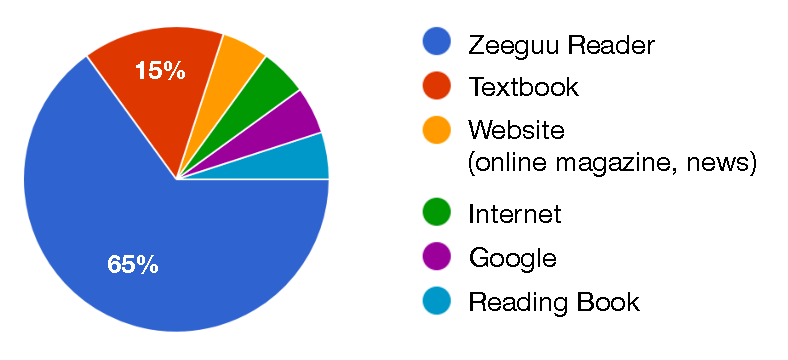
\includegraphics[width=0.6\columnwidth]{figures/opinions/reader_vs_textbook.pdf}
      \caption{Answers to the question: {``If you wanted to read something in the language you study, what would you reach out for first?''}}
      \label{fig:preferred_reader}
    \end{figure}



\subsection{About The Exercises}
Figure \ref{fig:ex_rating} shows that when asked to provide their personal rating of the the quality of the exercises, the majority of the respondents are positive: 

 \begin{figure}[h!]
    \centering
      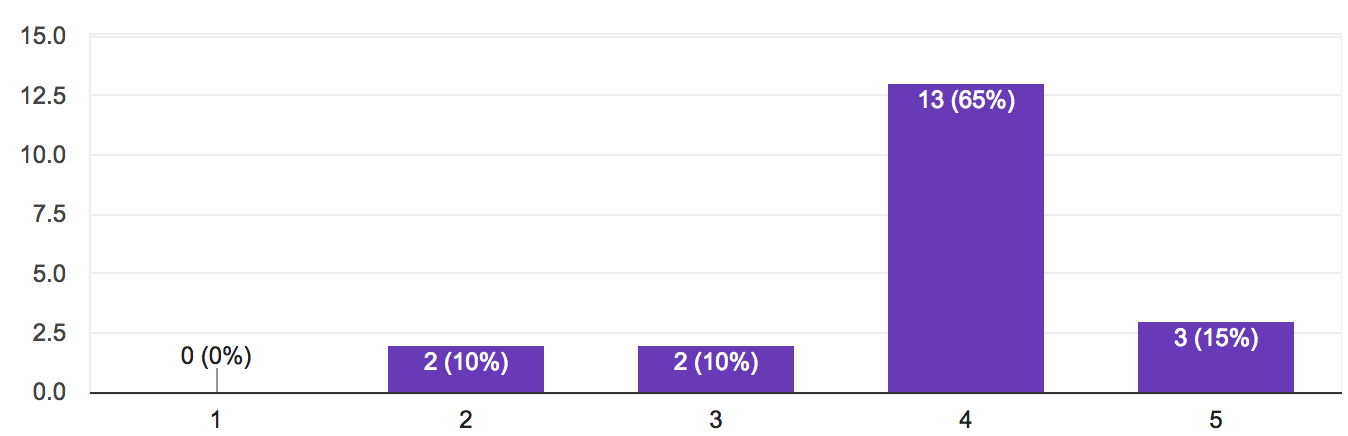
\includegraphics[width=0.8\columnwidth]{figures/opinions/exercises_rating}
      \caption{Students assessment  of the generated exercises}
      \label{fig:ex_rating}
    \end{figure}

When asked about what they dislike about exercises, many said literally ``nothing''. However, several also had concrete feedback that can be classified in two main directions: 

\begin{enumerate}

  \item Contexts are always the same: \squote{I would like to see the words I practice in a different context}. This would indeed be an idea worthy of further investigation.

	\item Exercises can be too easy. One learner wrote in their feedback that \squote{some exercises are too easy}. 

  \item Exercises can be too difficult. Some learners encountered exercises in which they did not understand well the context, and would have wanted translations for it. However, translations are not enabled during exercises, so they reported that: \squote{There aren't translations}, \squote{Doesn't give the translations}. 
	
\end{enumerate}

\subsection{About The Overall System}
% During the running of the experiment, randomly selected students were asked a series of questions by popping up questions while they were using the system. For this, we used an online tool called HotJar. Among the questions was whether they preferred the reading platform and why. Some of the answers can be seen in the screenshot below. It becomes clear that the students appreciate the possibility of reading what is interesting for them.

%     \begin{figure}[h!]
%     \centering
%       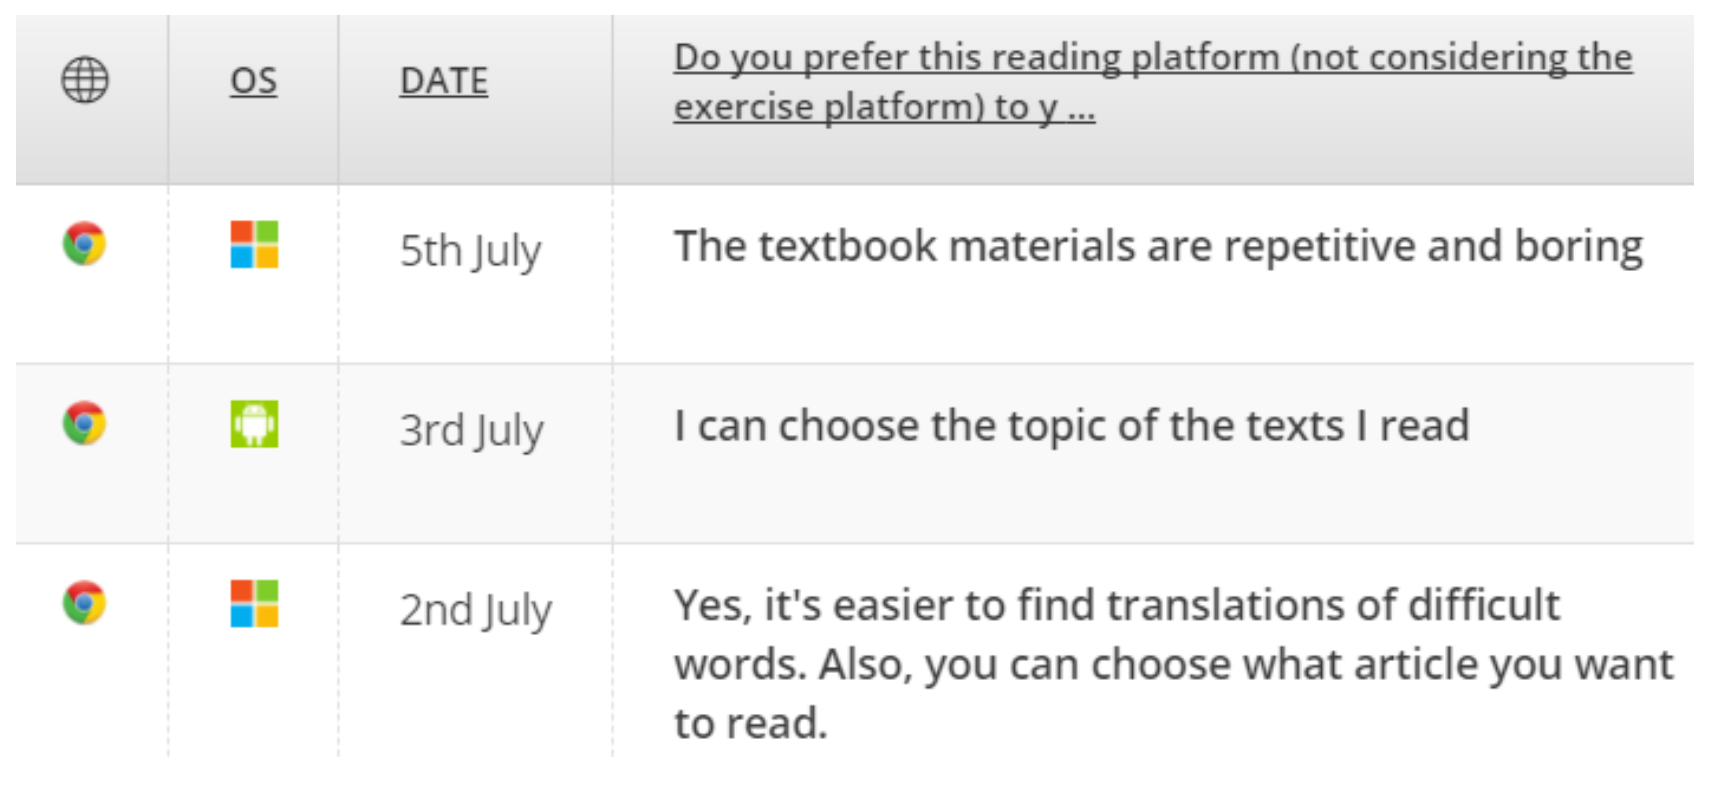
\includegraphics[width=0.7\columnwidth]{figures/opinion_on_reading_platform}
%       \caption{The students appreciate the freedom of choosing what to read}
%     \end{figure}


% \newpage
% \subsection{Reports to the Teacher}
At the end of the semester, the students had to provide feedback to their teacher about all of the software tools they used in the class during the year. This is something that the teacher always does at the end of the school year. Since the students had to write also about our system, we asked the teacher if we could access the corresponding feedback and they were glad to oblige. 

Six students wrote more detailed opinions. The main ideas in the feedback are illustrated by the three example quotes listed below\footnote{Although the original feedback is in Dutch, we translated all the  detailed answers and uploaded them online in the associated data repository of the paper as {\em feedback-to-the-teacher.txt}}: 

\begin{description}
  \item {\em ``It's good for improving reading skills. It would be even better if this tool was available in Dutch''}
  \item {\em ``Works well, but if it were possible to translate to Dutch it would have been better. Good that you can choose what you read.''}
  \item {\em ``My vocabulary truly is improving, but you do have to use it more than a few times. A very nice website, easy to use and with nice topics''}
\end{description}


Thus, learners appreciate the freedom of choosing materials to read that are personally interesting for them. They also appreciate the translations, but they would want to have them in their native language. 


% The way forward is then, by providing better recommendations if possible, and by providing translations in their native languages.

% In the future we plan to investigate whether the system works well enough with Dutch.

%!TEX root=paper.tex

\newcommand{\q}[1]{($Q_#1$)}
\newcommand{\qq}[2]{($Q_#1,Q_{#2}$)}

\newpage
\section{The Perception of the Teacher}
% \section{What Is the Perception of the Teacher?}
After the deployment at the school was finished we conducted a semi-structured interview with the language teacher of the three classes to gain insight into his perception of the benefits and limitations of the system. 
% 
The teacher, who self-describes as {\em an experienced teacher and language scientist as well}, argues that: 

\begin{itemize}

	\item [-] Such a system is critical for language education in schools, since the possibility of choosing their topics of interest is motivating for the students, and motivation is critical \q{3}\footnote
		{The $Q_n$ annotations refer to the questions in the full text of the interview, found  in the data repository as: {\em teacher-interview.txt}}. 

	\item [-]The system should be used for students who had already two or three years of foreign language experience \q{5}. 

	\item [-]There is no danger that every student will develop his little individual vocabulary bubble. Once the students have a solid basic vocabulary, it is perfectly acceptable that they study the words which interest them. \q{5}

	\item [-]The used sources were maybe too general. One source which was very focused on sport news was found very interesting by several students, mostly boys. More highly specific sources for other topics could be good \q{7}.

	% \item usually I made them learn vocabulary by heart for a test but this has proven to be rather useless because it only improves their short-term memory.  the good thing about your system is that they encounter a lot of words a lot of times and also you have spaced repetition and that is very good for learning vocabulary


	\item [-] It is ``more than acceptable'' that the translations are not perfect and every now and then a student must look up an alternative translation. This might help students become more actively engaged with the texts \q{9}. 
	% If 98% of the translations are correct they only click on the world and they continue reading but when they look at the word and have to think about whether is the right translation or not, they are more active. You

	% 
	% students have been studying French for 3 years the most frequent vocabulary they already have. I am an experienced teacher and language scientist as well; I know that when you have this base vocabulary and you go beyond it most of the world that just in the text are still the same, a small proportion of the words the people use. If you look at the French language, there are 25’000 words but when you're reading an article, you only encounter very few of those 25’000 words. When students read different texts, I think in the end 75% of the words that they will learn will be the same. 

	\item [-]The most important missing feature of the system is the possibility of comprehensively verifying that the students put quality and time in using the system at home \qq{2}{11}.

\end{itemize}


The teacher decided to extend the use of the system during the academic year 2017--2018 with a larger group of students. 
% However, not all the new classes are bilingual, we will have to explore the best approach for situations in which the L1 is not English but Dutch.

%!TEX root=paper.tex

%!TEX root=paper.tex

\section{Lessons Learned}

% \subsection{Reading Personalization Works And Learners Want More}
\subsection{Learners Appreciate Personalization But More Is Needed}
Based on telemetry, we confirmed that the opportunity of reading personalized materials is used by the students. Also in their feedback, students appreciate highly the personalization of reading content. The teacher thinks that student motivation is increased due to the possibility of reading texts they like. 
% 
However, one of the recurring themes of the student feedback is the need for a better way to find personally interesting articles. One possibility is suggested by the learners: the possibility of browsing articles by topics rather than sources. Another is a recommender system that takes as input the learner feedback on existing articles (e.g. the use of the Like button).
% An even more advanced system could try to automatically recommend texts based on the past reading history of the learner the way music and book recommender systems work. 

% The way we did difficulty ranking was sub-optimal. Most of the difficulties were very close to each other in value, between 1 and 4 and they were generic instead of being personalized. We think that as a result, the difficulty estimations that the system presented were too abstract for the readers. And as a result, 


% This situation could happen either because our current difficulty computation is not good enough, or because the way it is presented in the user interface is not clear enough for the readers.

% One of the limitations of our difficulty computer, but also of other traditional readability metrics \cite{Kincaid75-Readability} is that they 

% A more advanced strategy is needed, one that is less abstract, and personalized for the individual learner. One approach would be to estimate the number of words that are likely to be unknown in an article for a particular learner. A complementary information about the article could be the number of words that we know are being learned at the moment which are to be found in that article. In this way, a learner can choose a text that also gives them the chance to re{\"e}ncounter words being learned. 


% \subsection{Personal Study Preferences}
The vocabulary practice scheduler tries to optimize the times when the words are being repeated based on the state of the art in spaced repetition. However, we received multiple requests from learners who want to practice the words in a given text, once they are finished reading it, in the vein of traditional textbooks. The ideal system would allow the learners to personalize the vocabulary scheduling algorithms. 


\subsection{Improving Text Difficulty Reporting}
One of the learners reported: \squote{My level of the language is quite low for now, so I clicked to get a translation very often. Too often.}. Since the feedback was anonymous, it is not clear whether this situation came about due to the limitations of the difficulty computation, the limitations of the user interface, or because the student was simply not as advanced as their colleagues. In any case, a more personal approach to difficulty computation and reporting seems to be needed in order to steer students away from articles which are too difficult for them. 


\subsection{Ensuring the Quality of Content}
As opposed to a traditional textbook, a personalized textbook like the one we present has no editors and no quality control. In our study we limited the possible sources of articles together with the teacher. Even so, one of the students, wrote in their feedback: {\em ``I would like to avoid articles which have information about accidents with human casualties''}. Ideally, this kind of personal preferences can be specified by the readers. One possibility would be integrating  foreign language search, as Lappas and Vlachos propose \cite{Lapp12-NonNative}. Another is crowdsourcing where learners (and teachers, or more generally, trusted advanced learners) can provide feedback on existing materials. Crowdsourcing has been identified by Heffernan et al. as one of the driving technologies in learning \cite{Heff16-crowdsourcing}. 

\subsection{Limitations of Automatically Generated Exercises}
% Another situation where the quality of non-human-selected material matters is the automatic extraction of the context to be used in exercises. 
Although it is practical and effective to reuse the original context of a word in exercises\cite{nagy95-context}, sometimes the context in which the learner looks up a word is too long, sometimes too short, sometimes too difficult, and sometimes too easy. Estimating the quality of the automatically extracted context of an exercise, and ensuring that it is in the {\em zone of proximal development} -- where they are not too easy, and not too hard \cite{Zaretskii09-ProximalDevelopment} -- is a challenge for future builders of similar systems. 
 % must address.
 % One measure that we are considering is: ensuring that all the words in the context are simpler than the tested word. 



\subsection{Insight Into Student Activity Is Important}
One of the advantages of our (eco)system architecture in comparison to other alternatives for online reading (e.g. browser extensions for translations) is that it allows the teacher to gain insight into the reading activity of students. The deployed system has a teacher dashboard showing a chronological list of the words that a student looked up in context. In the final interview, the teacher observed that the biggest missing aspect of the system is a more complete insight into student activity, in particular the time students spend and the quality of their work. What other kinds of information are critical for teachers and how to collect and present them is an open question.

% Such a system should present more advanced analytics that could enhance the teacher's understanding of the class. This is something that is a clear opportunity when moving to a digital textbook. 





% % \newpage
% \section{Challenges}
% \label{sec:challenges}

% In this section we explore some of the challenges that we perceive need to be addressed by our system and similar ``personal textbook'' systems. We base our list of challenges on our observations and on the feedback that we received from our learners. The full list of recommendations from our users can be found in the GitHub repository online.

% \subsection{Registering for ``topics'' instead of ``sources''}
% Multiple learners asked for the possibility of registering to article topics rather than ``article sources''. A future system should consider this.


% \subsection{The selection of vocabulary to study}

% How do we automatically verify the ``learnability '' of an example in the context? It is a great responsibility automatically selecting a word to study. The situation where a user accepted a mistaken translation, and then the system ``teaches'' the learner that word would be disastruous. Currently we have a set of filters that try to avoid this, moreover, we also offer the learner the possibility of providing feedback in case he is not confident in a given translation. In the future, we consider using crowdsourcing to decrease even more the probability of wrong translations.
% \ml{alternate perspecitve: Do the learners choose the right translation? }% 	\item provide shorter sentences



% A few other types of improvement ideas that we have received from our beta-testers are: 
% \begin{itemize}
% 	\item be forgiving with misspellings, allow retry if the learner was close instead of considering it a mistake
% 	\item better provide hints than simply showing the answer
% \end{itemize}


% \subsection{Evaluating the quality of examples}

% It is indeed desirable to find good examples of practice exercises from past readings. Sometimes, the context in which the learner looks up a word is too long and sometimes it is too short. How to estimate the quality of an exercise? One measure that we are considering is: ensuring that all the words in the context are simpler than the tested word. 

% For beginners, this is still not an option. So we can only do this for students who are already quite advanced. \todo{We should see whether there's a difference between the ones that were A2 vs. B1}

% \subsection{Estimating article difficulty in a personal way}
% The way we did difficulty ranking was sub-optimal. Most of the difficulties were very close to each other in value, between 1 and 4 and they were generic instead of being personalized. We think that as a result, the difficulty estimations that the system presented were too abstract for the readers. And as a result, one of the readers reported that he disliked about the Reader the fact that \squote{My level of the language is quite low for now, so I clicked to get a translation very often. Too often.} 

% A more advanced strategy is needed, one that is less abstract, and personalized for the individual learner. One approach would be to estimate the number of words that are likely to be unknown in an article for a particular learner. A complementary information about the article could be the number of words that we know are being learned at the moment which are to be found in that article. In this way, a learner can choose a text that also gives them the chance to re{\"e}ncounter words being learned. 


% \subsection{Investigating more possible classroom workflows}
% The system was initially designed for self study. However, when invited to test it in a formal classroom we were happy to oblige.


\section{Limitations of the Study}
\label{sec:limitations}
% We presented a system, and we showed that it has the potential to generate user involvement. However the study we performed is not sufficient to reach a strong conclusion about the impact of the system we present... 

% The feedback from the users was overall positive, with many of them showing appreciation for the personalization aspects of the system. 
Although results are promising, further studies are needed since there are multiple reasons for which these results might not extend to the broader population. 
The students might have been influenced by our enthusiastic presentation of the system at the beginning of the testing month. 
Also, the students we worked with are not necessarily representative for the Dutch highschool student population since they are bilingual. 
% Even in this case, during the feedback multiple of them remarked that they would prefer to use the system in their native Dutch as opposed to English.
Also, the number of students who answered our survey was limited: only \surveyrespondents students which represents only about 30\% of the participants who actually used the system.

% We showed that the majority of the students used the system constantly throughout the one month period. 
% However, this might be because the students were encouraged to use the system as part of their assignment in the class. 
% If they used it only for the final grade, we would have expected a more focused cramming at the end of the period (which we actually saw with few of the students...). 


% We observed that students prefer to interact with different texts...  

% The algorithms for scheduling vocabulary exercises are the state of the art in spaced repetition. However, we did not have a control group to see whether this approach works better than others. Moreover, note that other approaches for using spaced repetition already exist; what is unique in our approach is that the students learn based on personalized exercises generated based on the context of their past readings.

Student interaction with texts and exercises indicates that at the end of the month they have learned words that they did not know at the begining and strengthened words they were not sure of. However, it is not clear whether this knowledge will remain for the long term. Currently only once a student has correctly handled a word three times in a row in exercises the system considers it learned and removes it from the exercises (even if it should probably be verified once more much later).

We encountered an enthusiastic teacher who thinks that such a system is critical to his classroom. Although we think he is right, he might not be representative of the general teacher population so more studies with language teachers are needed.


\section{Availability of The System, Code and Data}

% \subsection{Software}
The system described in this paper is deployed and available online. If the readers of this article want to test it they can use the {\em CHI2018} invite code while following the  ``Become a Betatester'' link at \url{https://zeeguu.unibe.ch/}.

The source code is open under a MIT license and available online at \url{https://github.com/zeeguu-ecosystem}. The code is covered by tests and documentation. To replicate a study like the one presented in this paper with another population, a researcher can deploy their own version of the system. 

% \subsection{Data}
Telemetry data representing all the interactions of the learenrs with the system, all student feedback, and a full transcript of the teacher interview are available on GitHub at: \url{https://github.com/zeeguu-ecosystem/CHI18-Paper}. 
% The same link holds the full anonymized questionnaire data. % used in this paper.





\section{Conclusions and Future Work}
We presented a system aimed to be a minimal viable product for a personalized language textbook that uses the web as its content source. We deployed the system with \studs high school students for one month. 
Based on telemetry we see that students take advantage of the possibility of personalization by 
  reading articles that are interesting and 
  by practicing words in exercises generated from their past readings. 
Based on their interactions we can see that their vocabulary is enriched with new words and the knowledge of other words is strengthened.
% , and that by using the system their vocabulary improves. 
 % with new words and strenghened knowledge of words they were not confident about. 

In their feedback, the students appreciate the possibility of reading personally relevant texts and the ease of interaction with the texts that is provided by the Reader component of our system. However, they also want better ways to find personally relevant content. The teacher of the three classes thinks that such a system is critical for the modern classroom, but wants more detailed data about student activity within the system.

As future work we see two salient directions. First, more work with teachers is needed to better understand how to combine the individual focus of personalized textbook with the collective experience of the learners in a classroom.
% , since other classroom workflows than the one presented here could be possible. 
Second, improved content recommenders and difficulty estimators are needed in order to provide an even better personalization of content and thus increase learner interest and motivation.
% Indeed, new workflows and classroom activities must be discovered.

% We hope that the availability of the system, code, and the open data that we published will make it easy for other researchers to investigate problems related to 
% foreign language reading.


{\footnotesize
	{\bf Acknowledgements.} We thank the anonymous reviewers for very valuable feedback. We thank Sara Vanini and Mark Langheinrich for advice, 
	% , Marc Langheirich, Gabriela Marcu .
	 Wim Gombert and Jeroen van Engen for collaboration,
	 and Oscar Nierstrasz for hosting the system on the SCG servers.
}



% Balancing columns in a ref list is a bit of a pain because you
% either use a hack like flushend or balance, or manually insert
% a column break.  http://www.tex.ac.uk/cgi-bin/texfaq2html?label=balance
% multicols doesn't work because we're already in two-column mode,
% and flushend isn't awesome, so I choose balance.  See this
% for more info: http://cs.brown.edu/system/software/latex/doc/balance.pdf
%
% Note that in a perfect world balance wants to be in the first
% column of the last page.
%
% If balance doesn't work for you, you can remove that and
% hard-code a column break into the bbl file right before you
% submit:
%
% http://stackoverflow.com/questions/2149854/how-to-manually-equalize-columns-
% in-an-ieee-paper-if-using-bibtex
%
% Or, just remove \balance and give up on balancing the last page.
%

\newpage

\balance{}

% BALANCE COLUMNS
\balance{}


% REFERENCES FORMAT
% References must be the same font size as other body text.
\bibliographystyle{SIGCHI-Reference-Format}
\bibliography{mir-biblio/aslan}

\end{document}

%%% Local Variables:
%%% mode: latex
%%% TeX-master: t
%%% End:
